\documentclass[12pt]{report}
\usepackage{graphicx}
\usepackage{multirow}
\usepackage{tabu}
\usepackage{makeidx}
\usepackage[left=2.5cm, right=1.5cm, top=2.5cm, bottom=1.5cm]{geometry}

\begin{document}
    \tableofcontents
    {
        \centering\chapter*{Practical NO.1}
        \section*{AIM: Study and usage of OpenProj.}
    }

{\bf OpenProj} : OpenProj is an open source project management software�
application. OpenProj operates on multiple platforms including Windows, Mac, 
Linux and Unix.OpenProj is a free, open-source project management solution. 
OpenProj is ideal for desktop project management and supports opening Microsoft 
or Primavera files. OpenProj 1.4 is an open source desktop project management 
application. This application is an alternative to Microsoft Project.

OpenProj provides control, tracking and management of projects. To create a new 
project the only field required is the Project Name on the Create New Project 
window and the start date of the project can be change it if you don?t want to 
start the day that you?re creating your project. You can add tasks in the Gantt 
diagram providing the start and end dates of each task; also you can add 
information to each task such the predecessors and successors tasks, resources, 
notes, etc. One great feature is that provides the Work Breakdown Structure
 (WBS) to order and control the tasks of the project for people who manages 
projects this is a very important tool. Another great feature is the Resource

Breakdown Structure (RBS) to define the structure of the resources, teams, 
providers, etc. Task Usage and Resource Usage are features to control your project and provide a good track on it. The Report tool provides information about the current status of your project.

The features of OpenProj are as follows:-
\begin{description}
\item{\textbf{Gantt chart}}:- A Gantt chart is a type of bar chart, developed by Henry Gantt in the 1910s, that illustrates a project schedule. Gantt charts illustrate the start and finish dates of the terminal elements and summary elements of a project. Terminal elements and summary elements comprise the work breakdown structure of the project. Modern Gantt charts also show the dependency (i.e. precedence network) relationships between activities.

\item{\textbf{PERT graph}}:- The Program (or Project) Evaluation and Review Technique, commonly abbreviated PERT, is a statistical tool, used in project management, that is designed to analyze and represent the tasks involved in completing a given project. First developed by the United States Navy in the 1950s, it is commonly used in conjunction with the critical path method (CPM).

\item {\textbf{Resource Breakdown Structure (RBS) chart}}:- In project management, the resource breakdown structure (RBS) is a hierarchical list of resources related by function and resource type that is used to facilitate planning and controlling of project work. In some cases, a geographic division may be preferred. Each descending (lower) level represents an increasingly detailed description of the resource until small enough to be used in conjunction with the work breakdown structure (WBS) to allow the work to be planned, monitored and controlled.

\item{\textbf{Work Breakdown Structure (WBS) char}t}: - A work breakdown structure (WBS), in project management and systems engineering, is a deliverable oriented decomposition of a project into smaller components.A work breakdown structure element may be a product, data, service, or any combination thereof.

\end{description}


Steps of installation of OpenProj:
\begin{figure}[!th]
\centering

\includegraphics[width=0.7\linewidth]{images/image30.jpeg}
\caption{Download by clicking here}
\label{fig:image1}
\end{figure}
\begin{figure}[!th]
\centering
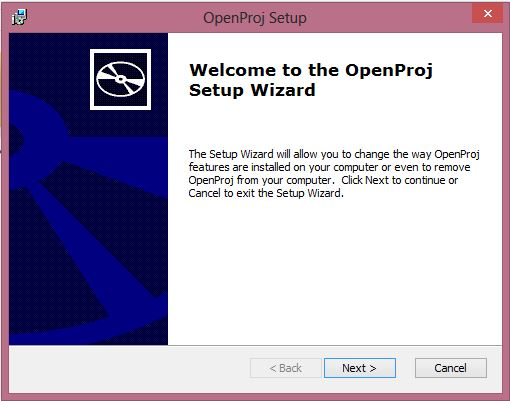
\includegraphics[width=0.7\linewidth]{images/image31.jpeg}
\label{fig:image1}
\caption{Run the executable file. Click Next in the welcome wizard.}
\end{figure}
\begin{figure}[!th]
\centering
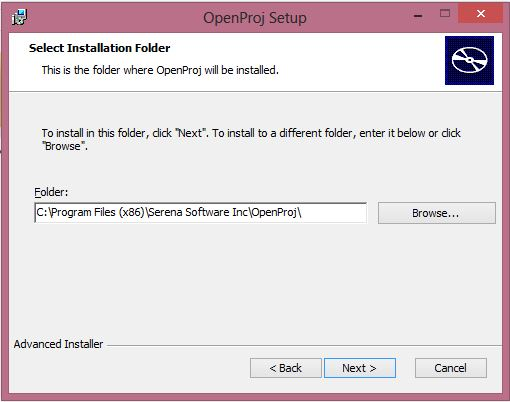
\includegraphics[width=0.7\linewidth]{images/image32.jpeg}
\label{fig:image1}
\caption{Click Install}
\end{figure}

\begin{figure}[!th]
\centering
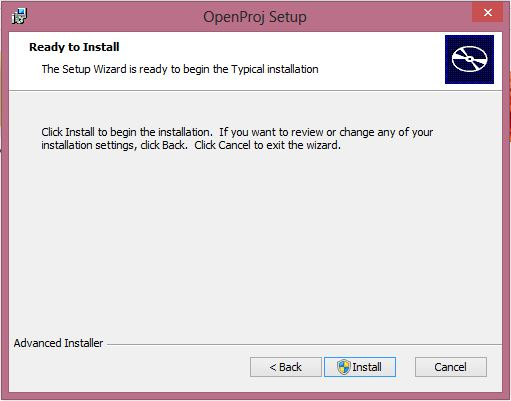
\includegraphics[width=0.7\linewidth]{images/image33.jpeg}
\label{fig:image1}
\caption{Click Finish}
\end{figure}

\begin{figure}[!th]
\centering
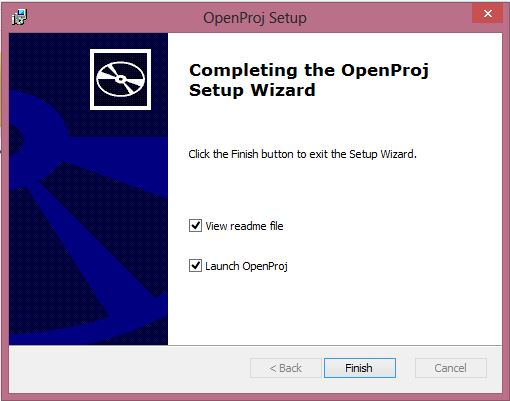
\includegraphics[width=0.7\linewidth]{images/image34.jpeg}
\label{fig:image1}
\caption{Create Project}
\end{figure}

\begin{figure}[!ht]
\centering
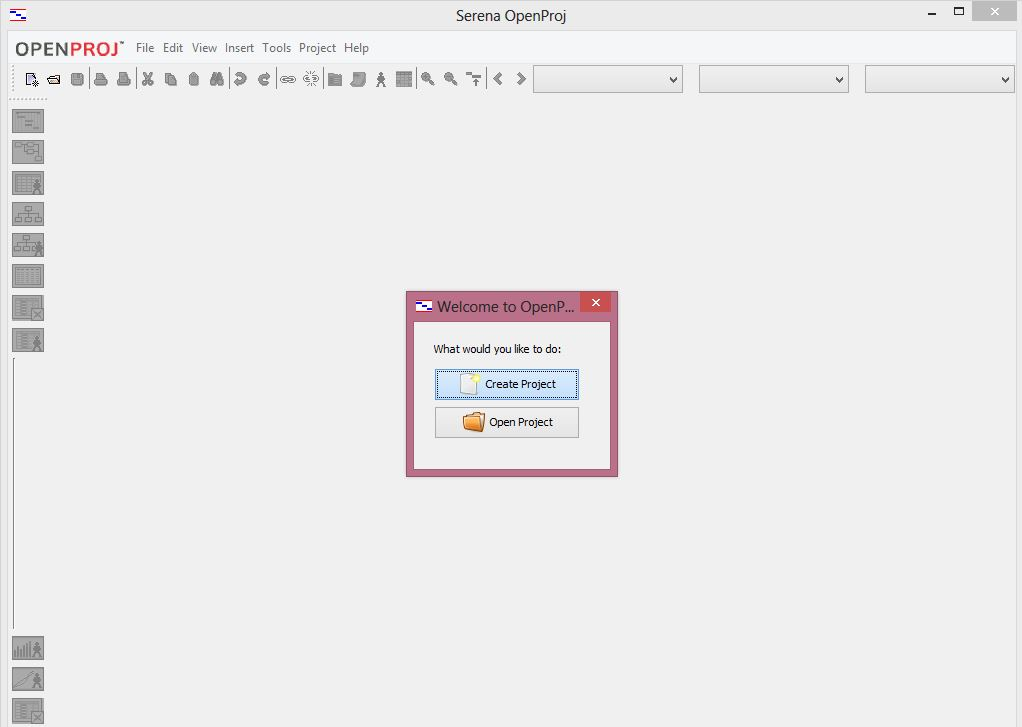
\includegraphics[width=0.7\linewidth]{images/image35.jpeg}
\label{fig:image1}
\caption{ Create Project Name: Structured Index model}
\end{figure}

\begin{figure}[!ht]
\centering
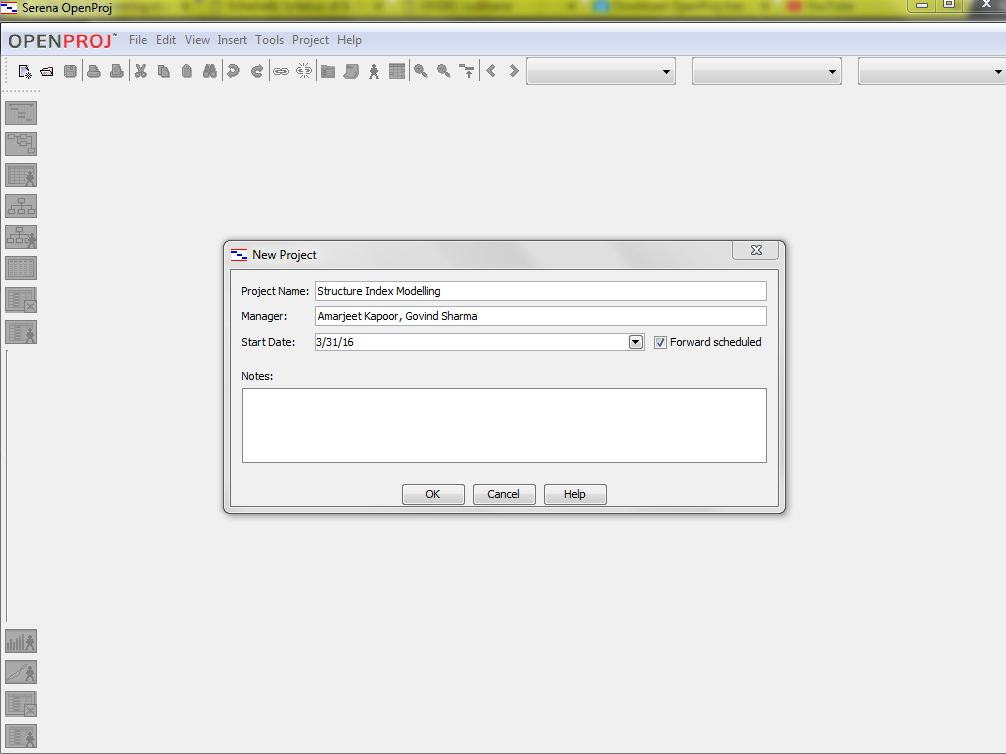
\includegraphics[width=0.7\linewidth]{images/image36.jpeg}
\label{fig:image1}
\caption{ Click OK}
\end{figure}

\newpage


{\centering
\chapter*{Practical NO. 2}
\section*{AIM: Study and usage of OpenProj to draft a project plan.}
}
To create projects in OpenProj Software:
\begin{enumerate}

\item Having downloaded and installed the OpenProj software; start OpenProj from the start menu of Windows or via the icon on your desktop. After the license agreement, OpenProj starts with a choice of creating a new project or opening an existing one. Choose ?Create Project?.



\item Enter a name for the project, the project manager?s name and a start date (which can also be modified later if required). Provide a description in the Notes section as you see fit.

\item The application window will be displayed consisting of following main components:- 
\begin{description}
\item{Indicator Column}:- In this column, symbols are displayed to show the status of the corresponding tasks (see right). 
\item{Task Number Column}:- Task numbers are assigned by OpenProj automatically when data is entered. The user does not enter information into this box. 
\item{Time Scale}:- In many views, OpenProj shows a timeline whose scale can be changed via the + and - magnifying glass icon on the menu above. 
\item{Information View Type}:- The area along the left side of the window lists a number of buttons representing the available views. Gantt, Network, Resources, WBS (work breakdown structure), RBS (resource breakdown structure), Reports, Task Usage and Resource Usage.  
\end{description}
\end{enumerate}
\begin{figure}[!ht]
\centering
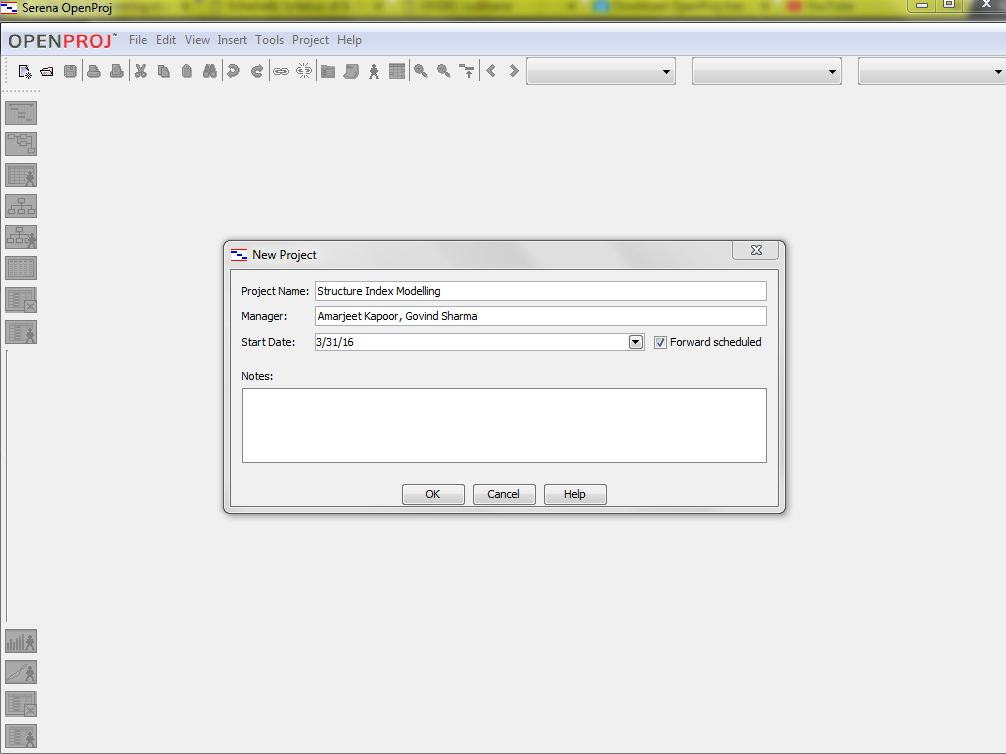
\includegraphics[width=0.7\linewidth]{images/image39.jpeg}
\label{fig:image1}
\caption{Creating Project}
\end{figure}
\begin{figure}[!ht]
\centering
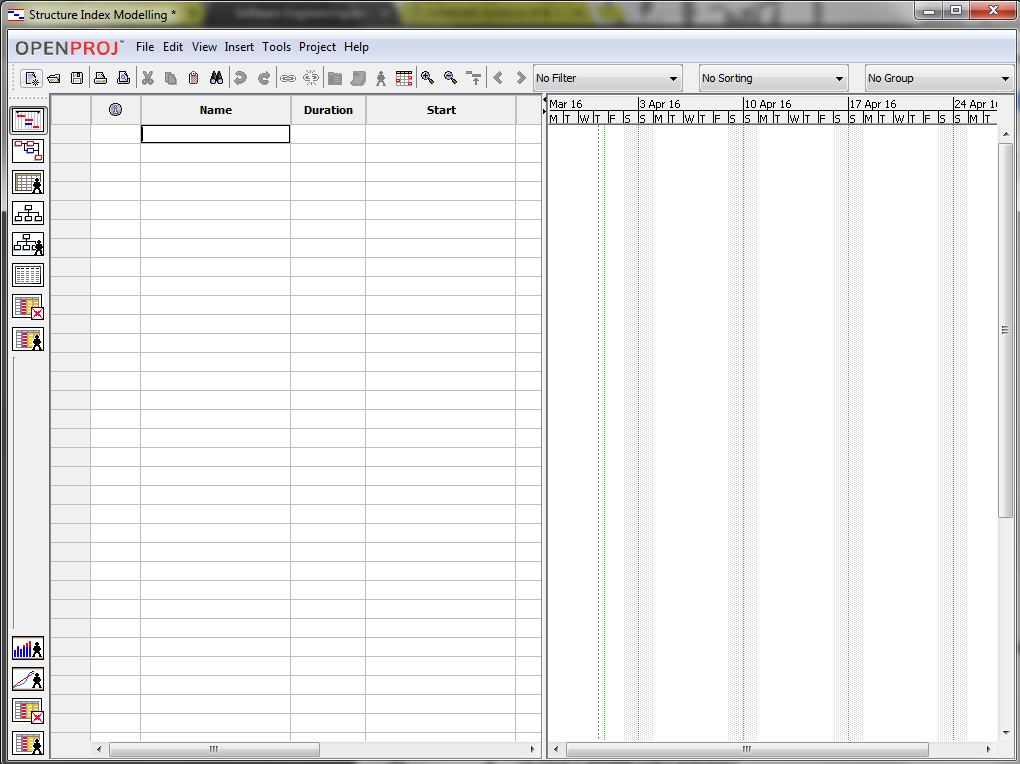
\includegraphics[width=0.7\linewidth]{images/2.JPG}
\label{fig:image1}
\caption{ application window}
\end{figure}
The lower view buttons open a split-screen where resource mapping tables and resource utilization as a graphic can be displayed. You can toggle views on and off by clicking the same button repeatedly.


\subsection*{To adjust the calendar while creating project in OpenProj Software:}
For accurate tracking of your project it is essential to first set up the OpenProj calendar to reflect the working hours in your organization. OpenProj offers three default calendars:
\begin{itemize}
         
\item Standard Calendar (Mon-Fri, 08:00 to 17:00 with 1hr lunch break at noon) 
\item Night Shift (Mon-Sat 23:00 to 08:00 with a 1hr break from 03:00 to 04:00) 
\item 24-Hour Calendar (24/7 schedule) 
\end{itemize} 
\begin{figure}[!ht]
\centering
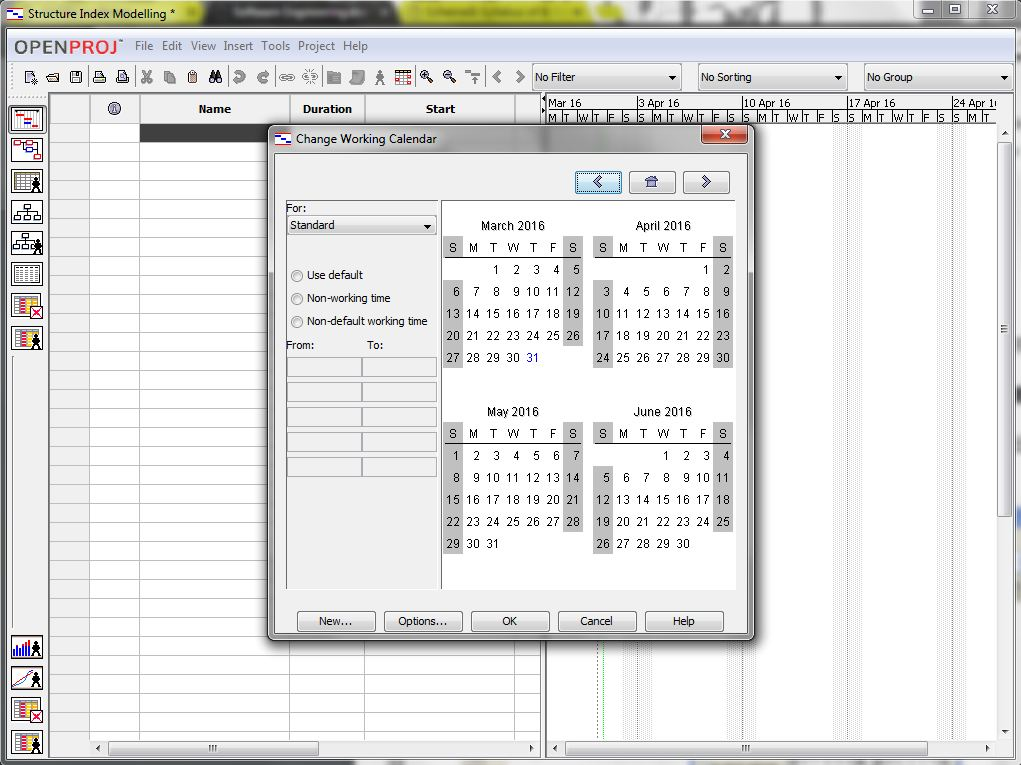
\includegraphics[width=0.7\linewidth]{images/3.JPG}
\label{fig:image1}
\caption{standard calender}
\end{figure}
\begin{figure}[!ht]
\centering
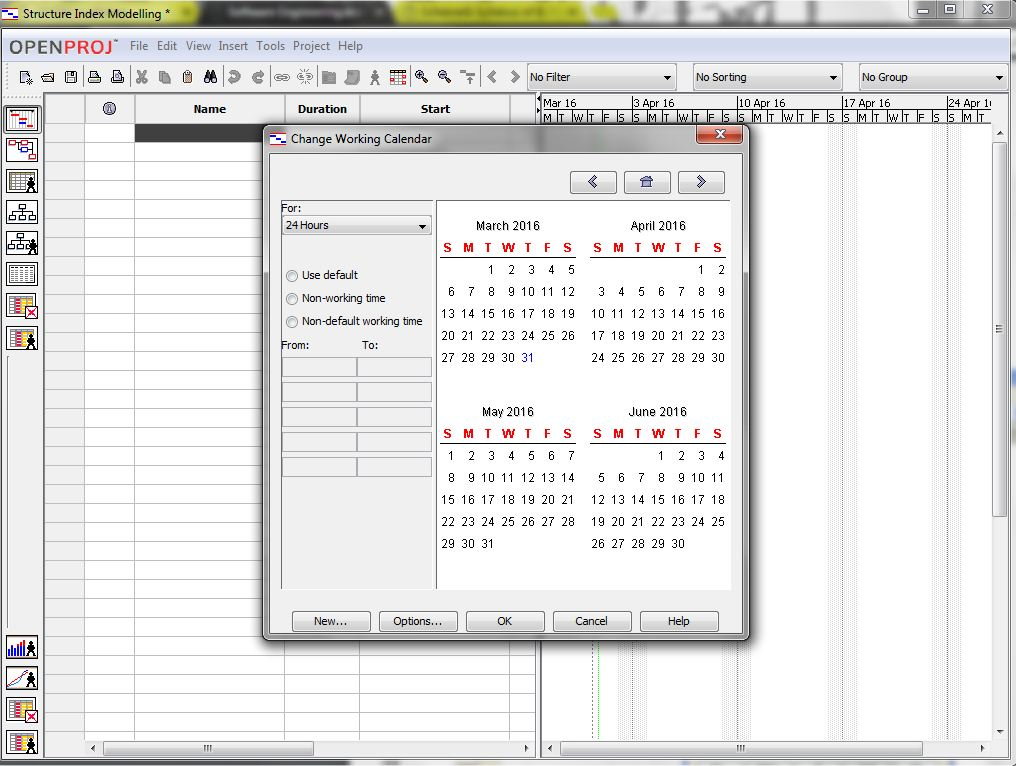
\includegraphics[width=0.7\linewidth]{images/4.JPG}
\label{fig:image1}
\caption{night calender}
\end{figure}
\begin{figure}[!ht]
\centering
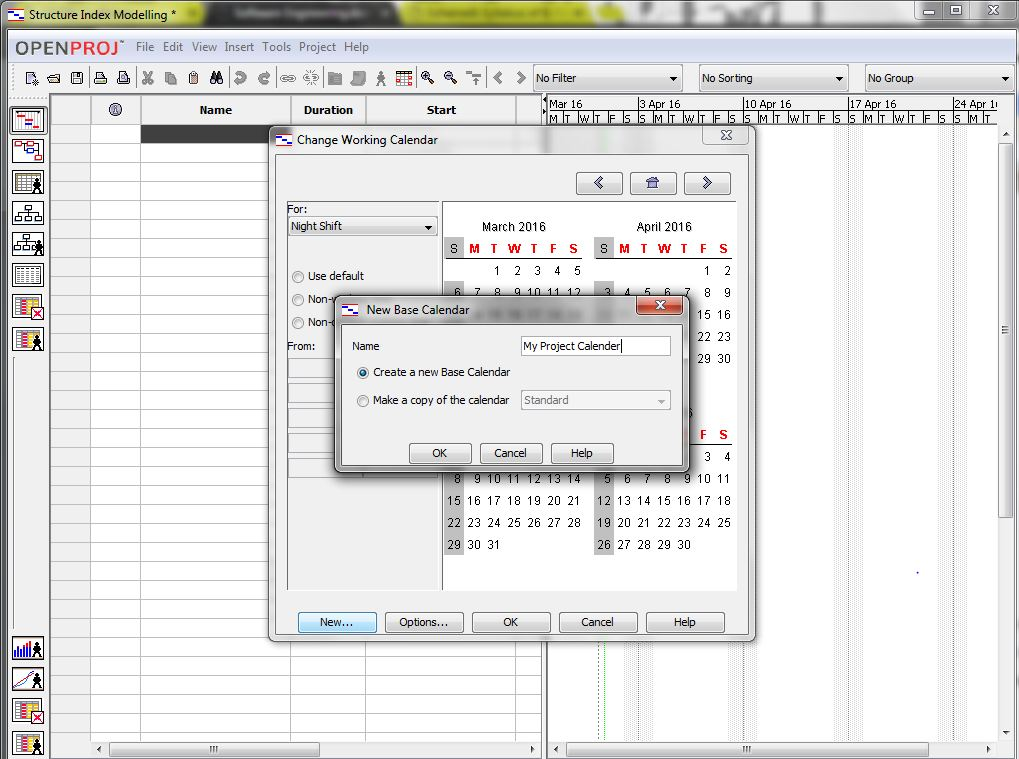
\includegraphics[width=0.7\linewidth]{images/6.JPG}
\label{fig:image1}
\caption{saving calender}
\end{figure}
We can assign any one of these to be your project calendar; however none of the default calendars contain public holidays so it is often necessary to create your own custom calendar to reflect your company's general working hours.
\begin{enumerate}

\item Open the Calendar with the menu tool Tools ? Change Working Calendar .

\item  Click on New to create a new calendar. 
\item Enter a name for your new calendar and click OK.
\item  Mark the days for which you want to change the working time (e.g. for all Fridays you can click the column header ?F?, or you can hold ctrl and click to select individual days). To make a global selection you would hold ctrl and click S,M,T,W,F,S in turn. 
\item  Click ?Non-default working time? on the left and change the working hours within the fields below.
\item  To mark company or public holidays, select the relevant days as above and click ?Non- working time?. 
\item  Edited calendar entries will appear in red. 
\item  Click ?Options? at the bottom to set the corresponding working hours per day, hours per week and days per month. If you do not do this, OpenProj will not schedule the tasks correctly. 
\item  Confirm changes by clicking OK.

\item You must now assign your custom Project calendar to your project. To do this, click Project ?Project Information from the top menu and set the Base Calendar to your new custom base calendar name. This is also the screen where you enter the Project Start Date. Click close when done.

\end{enumerate}

OpenProj can also associate calendars to individuals and to specific tasks. In this way you can designate individual vacation periods or you can specify a task to follow a different schedule to the one in your base calendar. So, in fact you can use three different types of calendars within your project: 

\begin{enumerate}

\item  Project calendar (your base calendar for the project as defined above) 
\item  Resource calendar (for individuals working time and vacation days)
\item  Task calendar (for tasks that do not follow the regular working hours, e.g. a task cannot start on a Friday because it would be interrupted by the weekend or maybe a task that runs continuously for 24hrs). 
content...
\end{enumerate}

The calendar is stored with the particular project file, so if you start another project it is necessary to create the user defined calendar again.


{\centering
\chapter*{Practical NO. 3}
\section*{AIM: Study and usage of OpenProj or similar software to track the progress of a project}
}

\textbf{To create Gantt Charts and Network charts in OpenProj Software:}
When you create a new project, OpenProj by default opens the Gantt chart view on the right pane and the task input table on the left pane. You can drag the vertical line dividing the two panes to fit your monitor as you desire. To enter a task: 
\begin{enumerate}

\item Click in the Name column in the first row. 
\item Enter a name for the task. 
\item Confirm the input by clicking the mouse or pressing the tab button which takes you to the duration entry field. 
\item If you do not know the duration at this stage you do not have to input it. OpenProj enters a default value of 1day? which you can alter at a later stage. 
\item If you have an estimate of the duration, then feel free to enter it into the cell. OpenProj automatically converts the duration to days. For example, enter 1w (1 week) and OpenProj will set the duration to 5 days. The input of 1 month would result in a display of 20 days and 1 hour would be displayed as 0.125 days (or 1/8th of a day). 
\item Confirm the input by pressing Enter or clicking on the next row. 
\item It is important that you enter only task names and durations at this stage. Do not be tempted to enter any other information right now. Especially a starting date. 
\item Its good practice even at this stage to enter general headings (phases) for tasks example ?Design? and then more specific tasks underneath, but never enter a duration for a general heading.
\end{enumerate}

\begin{itemize}

\item \textbf{Gantt Chart }
A Gantt chart, commonly used in project management, is one of the most popular and useful ways of showing activities (tasks or events) displayed against time. On the left of the chart is a list of the activities and along the top is a suitable time scale. Each activity is represented by a bar; the position and length of the bar reflects the start date, duration and end date of the activity. This allows you to see at a glance: 
What the various activities are 
When each activity begins and ends
How long each activity is scheduled to last 
Where activities overlap with other activities, and by how much 
The start and end date of the whole project 
To summarize, a Gantt chart shows you what has to be done (the activities) and when (the schedule).

\begin{figure}[!ht]
\centering
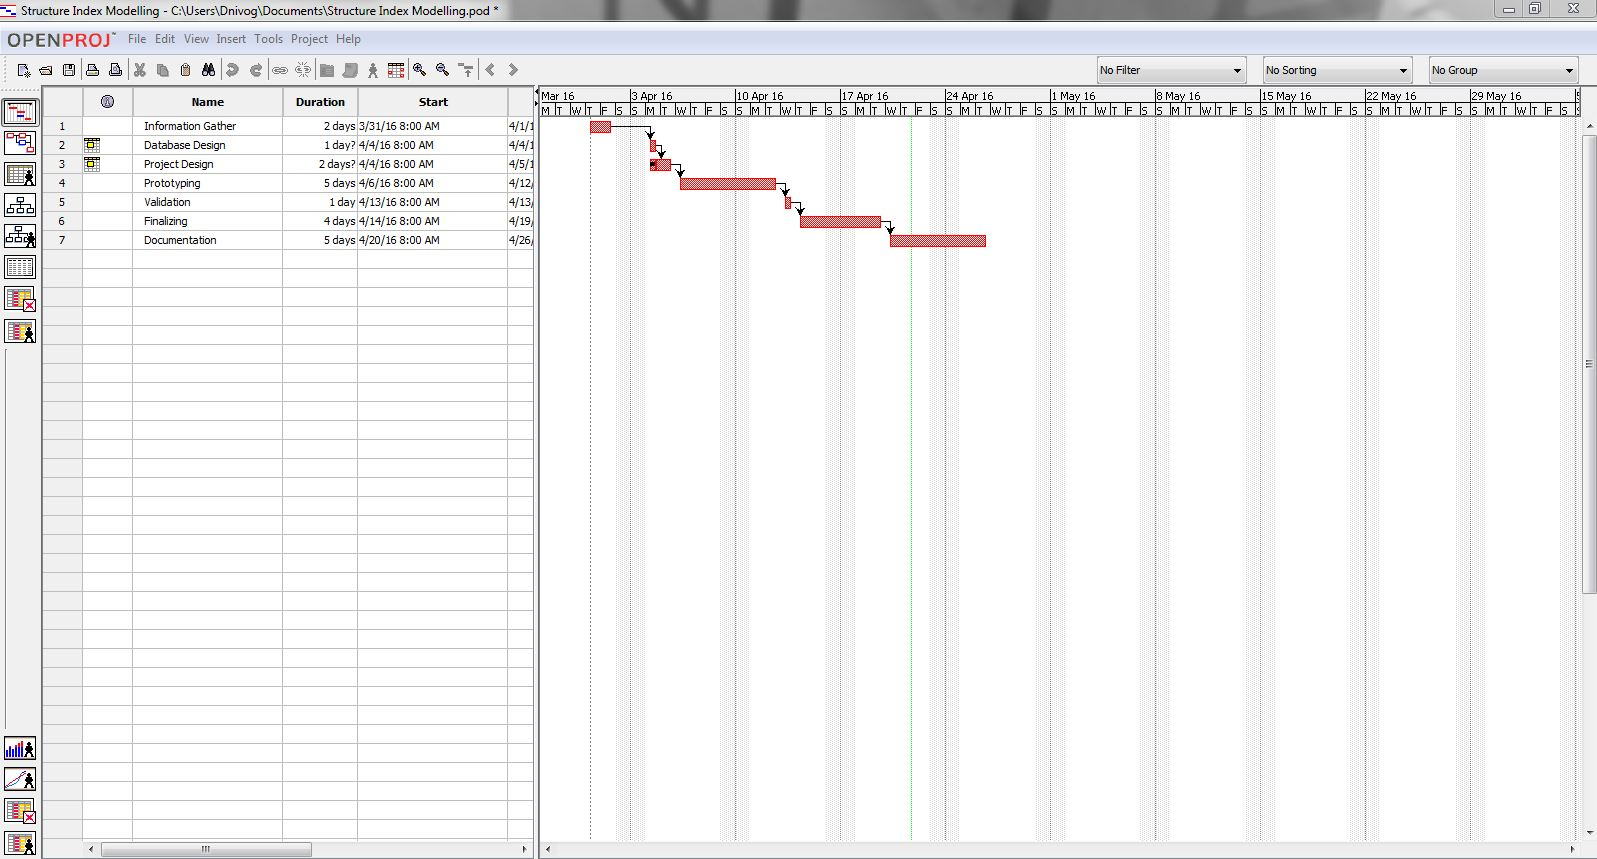
\includegraphics[width=1\linewidth]{images/image46.jpeg}
\label{fig:image1}
\caption{Gantt chart}
\end{figure}
                           
                                                                
\item\textbf{ Network Chart}
A network diagram is essentially a flow chart that includes all of the project elements and how they relate to one another. It shows parallel activities and the links between each activity. Network logic is the collection of activity dependencies that make up a network diagram for a particular project. In other words, certain tasks are dependent on one another to complete the project. This creates a logical stream of events that will lead to completion of the project. The network diagram lets you do the following:
\begin{itemize}
\item Define the project's path 
\item Determine the sequence of tasks to be completed 
\item Look at the relationship between activities 
\item Determine the dependencies 
\item Make adjustments as tasks are completed 
\item Take a broad look at the project path and clearly see the relationships and dependencies between tasks

\end{itemize}
CLICK ?View? and then ?Network diagram?. It will then generate the diagram shown below:


\begin{figure}[!ht]
\centering
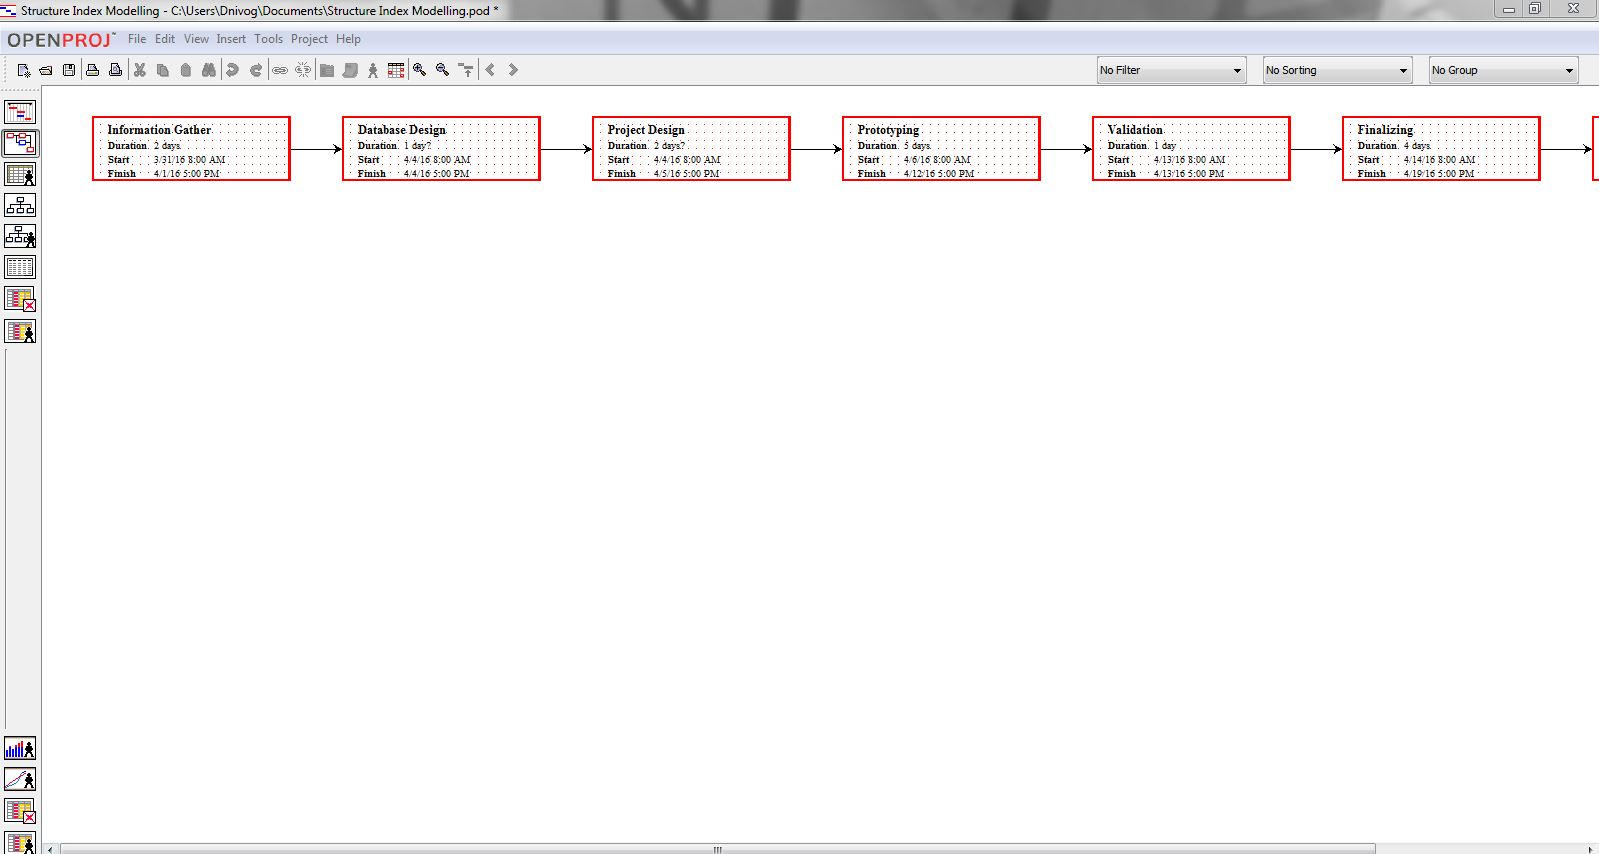
\includegraphics[width=1\linewidth]{images/image47.jpeg}
\label{fig:image1}
\caption{Network chart}
\end{figure}

                          
\item \textbf{Work Breakdown Structure(WBS)}
A�work breakdown structure (WBS), in�project management�and�systems engineering, is a deliverable-oriented decomposition of a project into smaller components. A work breakdown structure is a key project deliverable that organizes the team's work into manageable sections. The Project Management Body of Knowledge defines the work breakdown structure as a "A hierarchical decomposition of the total scope of work to be carried out by the project team to accomplish the project objectives and create the required deliverables."
A work breakdown structure element may be a�product,�data,�service, or any combination thereof. A WBS also provides the necessary framework for detailed cost estimating and control along with providing guidance for schedule development and control.


\begin{figure}[!ht]
\centering
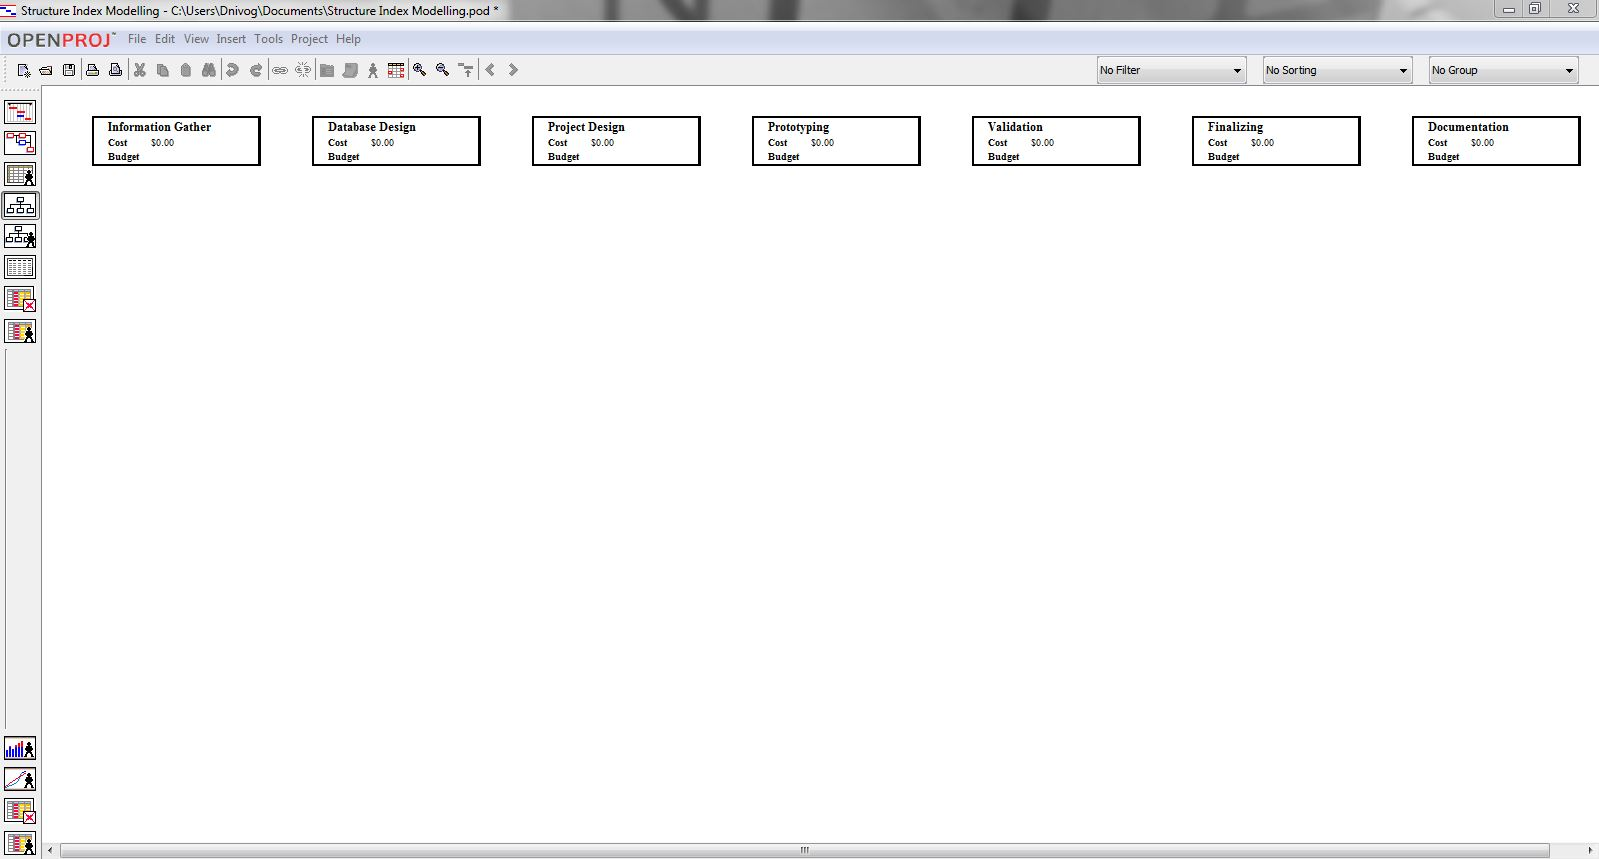
\includegraphics[width=1\linewidth]{images/image48.jpeg}
\label{fig:image1}
\caption{Work Breakdown Structure}
\end{figure}
\end{itemize}
\begin{figure}[!ht]
\centering
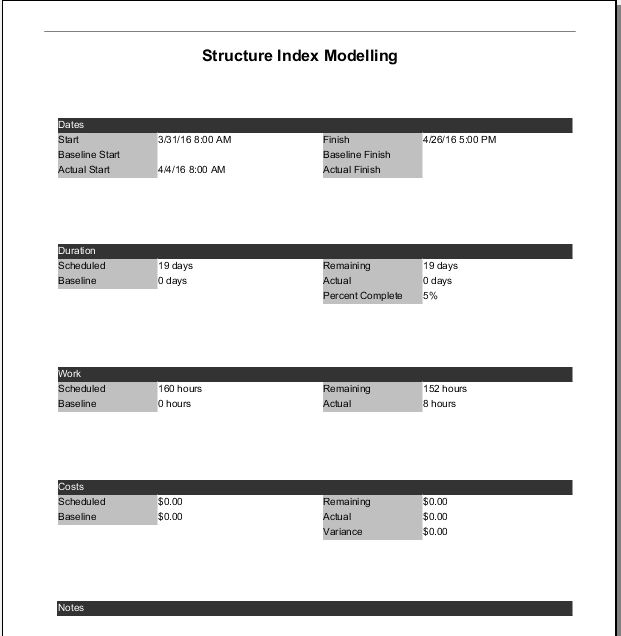
\includegraphics[width=1\linewidth]{images/image49.jpeg}
\label{fig:image1}
\caption{Report Chart}
\end{figure}

\begin{figure}[!ht]
\centering
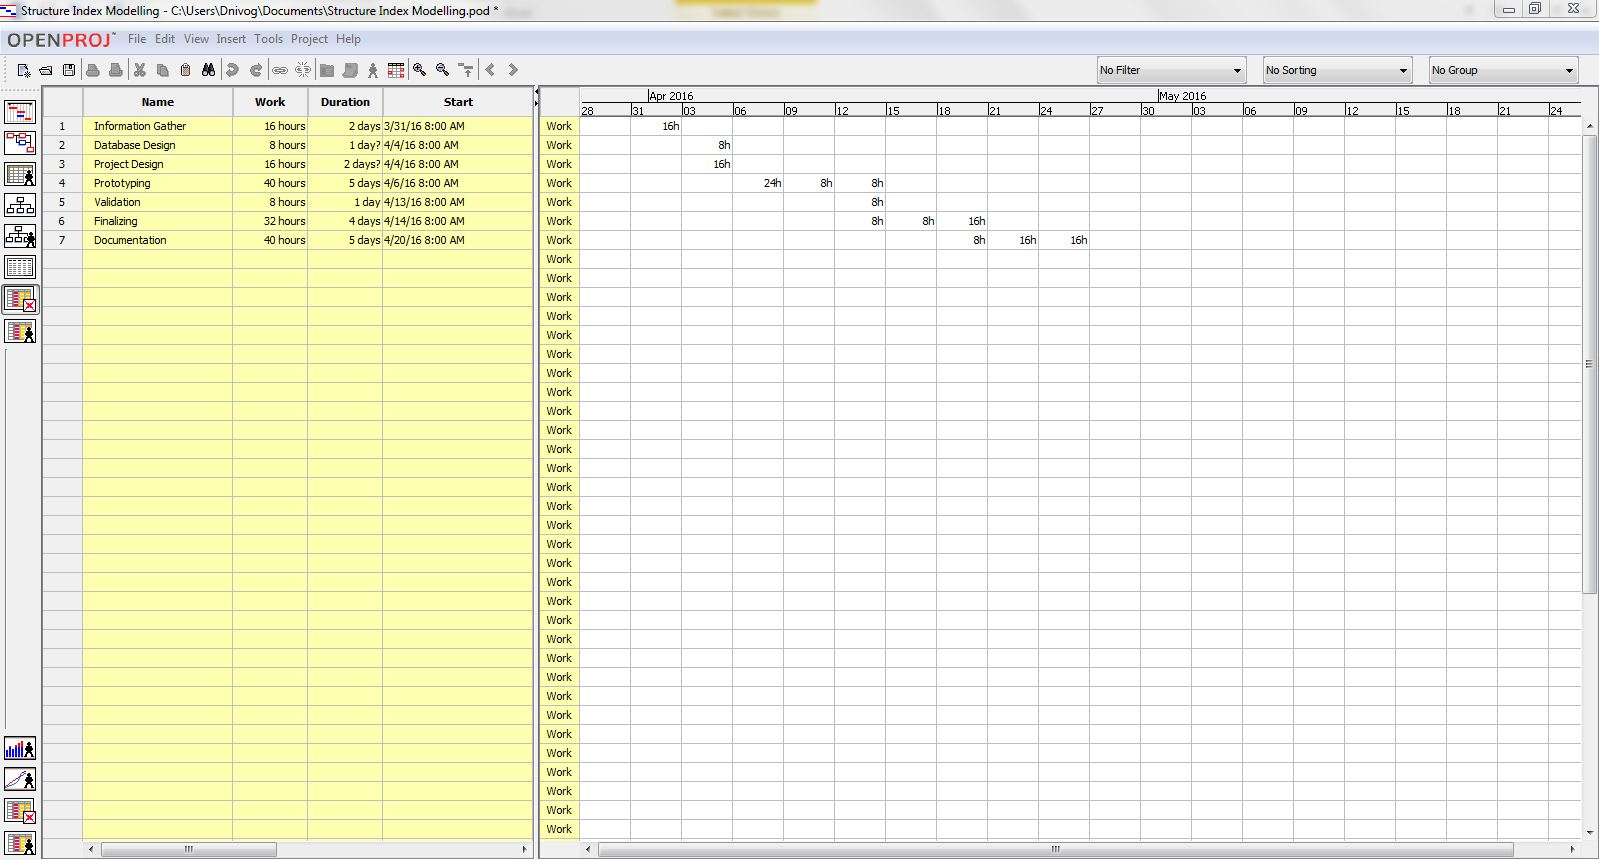
\includegraphics[width=1\linewidth]{images/image50.jpeg}
\label{fig:image1}
\caption{Task Usage chart}
\end{figure}


\textbf{
To set dependencies and establishes deadlines in OpenProj software}: 
Dependencies allow you to show the relationships between tasks and set rules for when tasks can be started or finished. OpenProj uses four types of dependencies:
\begin{description}

\item[FS (Finish-to-Start)]:- This is the default relationship in OpenProj. It defines that one task has to finish before the next one can start. For Example, ?printing a document? cannot start until ?editing the document? is finished. 
\item[SS (Start-to-Start)]:- The start of a task is dependent on the start of its predecessor. In other words, the task can only start after the predecessor task has started (or at a later date).
\item[FF (Finish-to-Finish)]:- The completion of a task is dependent on the completion of its predecessor. In other words, the task can only finish at the same time (or after) the previous task has finished.
\item[SF (Start-to-Finish)]:- The finish of the next task depends on the start of the previous task. In other words, the first task begins after the second task ends.
When dependencies are created, the start and finish dates of tasks are usually affected. OpenProj automatically edits start and finish dates so that they adhere to these new constraints. Any change to dependencies will update task dates and Gantt bars automatically.

\end{description}


{\centering
\chapter*{Practical NO. 4}
\section*{AIM: Preparation of Software Requirement Specification Document,
Design Documents and Testing Phase related documents for some
problems}
}


\subsection*{Software Requirement Specification Document}
An SRS is basically
 an organization's understanding (in writing) of a customer or potential
client's sy
stem requirements and dependencies at a particular point in time (usually
) prior to
any
 actual design or development work. It's a two-way
 insurance policy
 that assures that both
the client and the organization understand the other's requirements from that perspective at a
given point in time.

The SRS document itself states in precise and explicit language those functions and
capabilities a software sy
stem (i.e., a software application, an ecommerce Web site, and so
on) must provide, as well as states any
 required constraints by
 which the sy
stem must abide.
The SRS also functions as a blueprint for completing a project with as little cost growth as
possible. The SRS is often referred to as the "parent" document because all subsequent
project management documents, such as design specifications, statements of work, software
architecture specifications, testing and validation plans, and documentation plans, are related
to it.

It's important to note that an SRS contains functional and nonfunctional requirements only
; it
doesn't offer design suggestions, possible solutions to technology
 or business issues, or any

other information other than what the development team understands the customer's sy
stem
requirements to be.
A well-designed, well-written SRS accomplishes four major goals:
\begin{itemize}
\item
It provides feedback to the customer. An SRS is the customer's assurance that the
development organization understands the issues or problems to be solved and the
software behavior necessary
 to address those problems. Therefore, the SRS should be
written in natural language (versus a formal language, explained later in this article),
in an unambiguous manner that may
 also include charts, tables, data flow diagrams,
decision tables, and so on.

\item
It decomposes the problem into component parts. The simple act of writing down
software requirements in a well-designed format organizes information, placesborders around the problem, solidifies ideas, and helps break down the problem into
its component parts in an orderly
 fashion.

\item
It serves as an input to the design specification. As mentioned previously
, the SRS
serves as the parent document to subsequent documents, such as the software design
specification and statement of work. Therefore, the SRS must contain sufficient detail
in the functional sy
stem requirements so that a design solution can be devised.

\item It serves as a product validation check. The SRS also serves as the parent document
for testing and validation strategies that will be applied to the requirements for
verification.

\end{itemize}

SRSs are typically
 developed during the first stages of "Requirements Development," which
is the initial product development phase in which information is gathered about what
requirements are needed--and not. This information-gathering stage can include onsite visits,
questionnaires, survey
s, interviews, and perhaps a return-on-investment (ROI) analy
sis or
needs analy
sis of the customer or client's current business environment. The actual
specification, then, is written after the requirements have been gathered and analy
zed.
Why
 Technical Writers should be involved with Software Requirements Specifications?
Unfortunately
, much of the time, sy
stems architects and programmers write SRSs with little
(if any
) help from the technical communications organization. And when that assistance is
provided, it's often limited to an edit of the final draft just prior to going out the door. Having
technical writers involved throughout the entire SRS development process can offer several
benefits:
\begin{itemize}

 \item Technical writers are skilled information gatherers, ideal for eliciting and articulating
customer requirements. The presence of a technical writer on the requirements-gathering
team helps balance the ty
pe and amount of information extracted from customers, which
can help improve the SRS.
  \item Technical writers can better assess and plan documentation projects and better meet
customer document needs. Working on SRSs provides technical writers with an
opportunity
 for learning about customer needs firsthand--early
 in the product
development process.
 \item Technical writers know how to determine the questions that are of concern to the user or
customer regarding ease of use and usability
. Technical writers can then take that
knowledge and apply
 it not only
 to the specification and documentation development,
but also to user interface development, to help ensure the UI (User Interface) models the
customer requirements.
 \item Technical writers, involved early
 and often in the process, can become an information
resource throughout the process, rather than an information gathered at the end of the
process.
\end{itemize}
In short, a requirements-gathering team consisting solely
 of programmers, product marketers,
sy
stems analy
sts/architects, and a project manager runs the risk of creating a specification
that may
 be too heavily
 loaded with technology
-focused or marketing-focused issues. The
presence of a technical writer on the team helps place at the core of the project those user orcustomer requirements that provide more of an overall balance to the design of the SRS,
product, and documentation.
\textbf{What Kind of Information Should an SRS Include?}
You probably
 will be a member of the SRS team (if not, ask to be), which means SRS
development will be a collaborative effort for a particular project. In these cases, y
our
company
 will have developed SRSs before, so y
ou should have examples (and, likely
, the
company
's SRS template) to use. But, let's assume y
ou'll be starting from scratch. Several
standards organizations (including the IEEE) have identified nine topics that must be
addressed when designing and writing an SRS:

\begin{enumerate}

\item Interfaces
\item Functional Capabilities
\item Performance Levels
\item Data Structures/Elements
\item Safety

\item Reliability

\item Security
/Privacy

\item Quality

\item Constraints and Limitations

\end{enumerate}
\textbf{Begin with an SRS Template}
The first and biggest step to writing an SRS is to select an existing template that y
ou can fine
tune for y
our organizational needs (if y
ou don't have one already
). There's not a "standard
specification template" for all projects in all industries because the individual requirements
that populate an SRS are unique not only
 from company
 to company
, but also from project to
project within any
 one company
. The key
 is to select an existing template or specification to
begin with, and then adapt it to meet y
our needs.
In recommending using existing templates, I'm not advocating simply
 copy
ing a template
from available resources and using them as y
our own; instead, I'm suggesting that y
ou use
available templates as guides for developing y
our own. It would be almost impossible to find
a specification or specification template that meets y
our particular project requirements
exactly
. But using other templates as guides is how it's recommended in the literature on
specification development. Look at what someone else has done, and modify
 it to fit your project requirements. (See the sidebar called "Resources for Model Templates" at the end of
this article for resources that provide sample templates and related information.)

\subsection*{A sample of a more detailed SRS outline}
\begin{enumerate}
\item Scope  
	\begin{enumerate}
	\item An STAAD PRO parsing
		application using C++, My
		SQL,
		make, Doxy
		gen, HTML, Py
		thon,
		Shell script, CSV
		Sy
		stem overview.
		\item
		\begin{enumerate}
		\item  Getting and validating a
		STAAD PRO file through a web
		interface from the user. \\
		\item Parsing the STAAD Pro
		file and storing the information
		in the database. \\
		\item Processing the database
		based on the user queries and
		presenting the output.
		 		\end{enumerate}
		\item  Document overview.
		A civil engineer can use this
		project to infer some very
		 useful
		information in matter of seconds
		from the already
		 existent
		STAAD PRO file. At the same
		time the information is being
		stored in a database that can be
		made available to a community
		of engineers for research and
		reference.
		This document comprises six
		sections:
		\begin{itemize}
		\item Scope
		\item Referenced documents
		\item Requirements
		\item Testing and Coding 
				\end{itemize}
\end{enumerate}


\item Referenced Documents 
\begin{enumerate}
\item STAAD PRO technical
manual.
\item Material database.
\end{enumerate} 
\item Requirements 
\begin{enumerate}
\item An interface for navigating
through the various parts of a 3
dimensional structure.
\item Properly
 abstracted options for
queries on various elements of
the building using Structured
Query
 Language.
\item A web interface for uploading
files and excessing the processed
data from any
 sy
stem over the
web.
\item Flexibility
 to incorporate any
changes in the standard sy
ntax of
the STAAD PRO scripting
methods. 

\end{enumerate}
\end{enumerate}
\subsection*{Design Documents}
A software design document (SDD) is a written description of a software product, that a
software designer writes in order to give a software development team overall guidance to the
architecture of the software project. An SDD usually
 accompanies an architecture diagram
with pointers to detailed feature specifications of smaller pieces of the design. Practically
, a
design document is required to coordinate a large team under a single vision. A design
document needs to be a stable reference, outlining all parts of the software and how they
 will
work. The document is commanded to give a fairly
 complete description, while maintaining ahigh-level view of the software. There are two kinds of design documents called HLDD
(high-level design document) and LLDD (low-level design document).
\begin{description}

\item[HLD] - High Level Design (HLD) is the overall sy
stem design - covering the sy
stem
architecture and database design. It describes the relation between various modules and
functions of the sy
stem. data flow, flow charts and data structures are covered under HLD.
High Level Design gives the overall Sy
stem Design in terms of Functional Architecture
details and Database design. This is very
 important for the ETL developers to understand the
flow of the sy
stem with function and database design wise. In this phase the design team,
testers and customers are play
s a major role. Also it should have projects standards, the
functional design documents and the database design document also.
\item[LLD] - Low Level Design (LLD) is like detailing the HLD. It defines the actual logic for each
and every
 component of the sy
stem. Class diagrams with all the methods and relation
between classes comes under LLD. Programs specs are covered under LLD. This document is
need to do during the detailed phase, the view of the application developed during the high
level design is broken down into separate modules and programs for every
 program and then
documented by
 program specifications.
\end{description}

Software testing is an investigation conducted to provide stakeholders with information about
the quality
 of the product or service under test. Software testing can also provide an
objective, independent view of the software to allow the business to appreciate and
understand the risks of software implementation. Test techniques include, but are not limited
to, the process of executing a program or application with the intent of finding software bugs
(errors or other defects).


It involves the execution of a software component or sy
stem to evaluate one or more
properties of interest. In general, these properties indicate the extent to which the component
or sy
stem under test:
\begin{itemize}

\item meets the requirements that guided its design and development,
\item responds correctly
 to all kinds of inputs,
\item performs its functions within an acceptable time,
\item is sufficiently
 usable,
\item can be installed and run in its intended environments, and
\item Achieves the general result its stakeholder?s desire.

\end{itemize}

As the number of possible tests for even simple software components is practically
 infinite,
all software testing uses some strategy
 to select tests that are feasible for the available time
and resources. As a result, software testing ty
pically
 (but not exclusively
) attempts to execute
a program or application with the intent of finding software bugs (errors or other defects).
Software testing can provide objective, independent information about the quality
 of software
and risk of its failure to users and/or sponsors. [Software testing can be conducted as soon as
executable software (even if partially
 complete) exists. The overall approach to software
development often determines when and how testing is conducted. For example, in a phased
process, most testing occurs after sy
stem requirements have been defined and then
implemented in testable programs. In contrast, under an Agile approach, requirements,
programming, and testing are often done concurrently


Test documentation is the complete suite of artefacts that describe test planning, test design,
test execution, test results and conclusions drawn from the testing activity
. As testing
activities ty
pically
 consume 30% to 50% of project effort, testing represents a project within a
project. Testing activities must therefore be fully
 documented to support resource allocation,
monitoring and control. This page identifies the ty
pes of documents y
ou need to set up and
run y
our test program and summarizes their content.

\subsection*{Test Plan}
The test plan describes the testing process in terms of the features to be tested, pass/fail
criteria and testing approach, resource requirements and schedules.

\begin{enumerate}

\item Introduction
\item Test items
\item Features to be tested
\item Testing approach
\item Item pass/fail criteria
\item Suspension and resumption
\item Deliverables
\item Tasks
\item Environmental needs
\item Responsibilities11. Staffing and training needs
\item Costs and schedule
\item Risks and contingencies

\end{enumerate}
\subsection*{Test Design Description}
The Test Design Description refines the Test Plan's approach, identify
ing specific features to
be tested and defining the test cases and test procedures that will be used.
\begin{enumerate}

\item \textbf{Features to be tested}
\begin{itemize}
\item Test items covered
\item Feature or feature combinations to be tested
\item References to software requirements specifications and software design descriptions

\end{itemize}

\item \textbf{Testing approach}
\begin{itemize}
\item Testing techniques to be used
\item Method of analy
zing test results (e.g. automated or manual)
\item Reasons for selection of various test cases
\item Environmental needs of test cases
\end{itemize}

\item \textbf{Test identification for each feature to be tested provide:}
\begin{itemize}
\item Test procedure identifiers and descriptions
\item Test case identifiers and descriptions
\item The pass/fail criteriaFlow Chart Of StudentData Flow Diagram
\end{itemize}
\end{enumerate}

\subsection*{DFD}
A data flow diagram (DFD) is a graphical representation of the "flow" of data through an
information sy
stem, modelling its process aspects. A DFD is often used as a preliminary
 step
to create an overview of the sy
stem, which can later be elaborated. DFDs can also be used for
the visualization of data processing (structured design).

A DFD shows what kind of information will be input to and output from the sy
stem, where
the data will come from and go to, and where the data will be stored. It does not show
information about the timing of process or information about whether processes will operate
in sequence or in parallel

Data flow diagrams are also known as bubble charts. DFD is a designing tool used in the top-
down approach to Sy
stems Design. This context-level DFD is next "exploded", to produce a

Level 1 DFD that shows some of the detail of the sy
stem being modeled. The Level 1 DFD
shows how the sy
stem is divided into sub-sy
stems (processes), each of which deals with one
or more of the data flows to or from an external agent, and which together provide all of the
functionality
 of the sy
stem as a whole. It also identifies internal data stores that must be
present in order for the sy
stem to do its job, and shows the flow of data between the various
parts of the sy
stem.

Data flow diagrams are one of the three essential perspectives of the structured-sy
stems
analy
sis and design method SSADM. The sponsor of a project and the end users will need to
be briefed and consulted throughout all stages of a sy
stem's evolution. With a data flow
diagram, users are able to visualize how the sy
stem will operate, what the sy
stem will
accomplish, and how the sy
stem will be implemented. The old sy
stem's dataflow diagrams
can be drawn up and compared with the new sy
stem's data flow diagrams to draw
comparisons to implement a more efficient sy
stem. Data flow diagrams can be used to
provide the end user with a phy
sical idea of where the data they
 input ultimately
 has an effect
upon the structure of the whole sy
stem from order to dispatch to report. How any
 sy
stem is
developed can be determined through a data flow diagram model.

In the course of developing a set of levelled data flow diagrams the analy
st/designer is forced
to address how the sy
stem may
 be decomposed into component sub-sy
stems, and to identify

the transaction data in the data model.

\begin{figure}[!th]
\centering
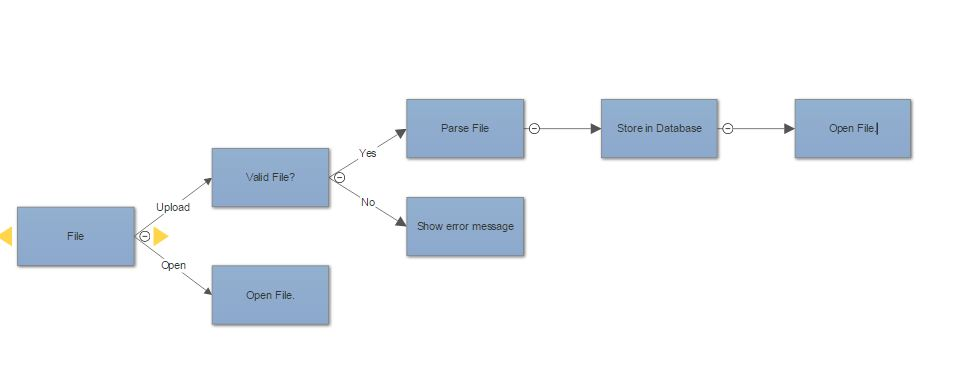
\includegraphics[width=1\linewidth]{images/image51.jpeg}
\caption{Decision Tree}
\label{fig:image1}
\end{figure}

\begin{figure}[!th]
\centering
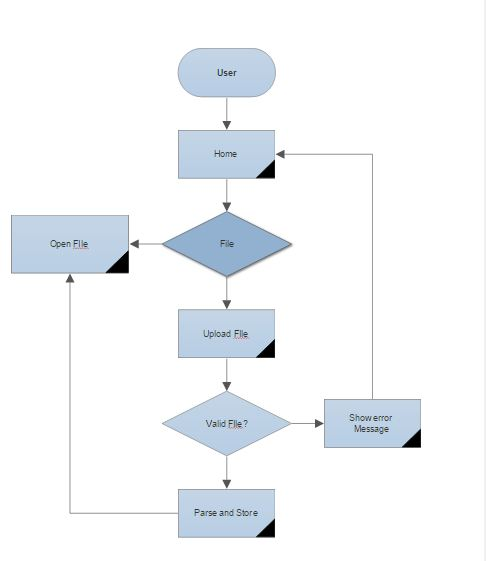
\includegraphics[width=0.7\linewidth]{images/image52.jpeg}
\caption{Flow Chart of SIM}
\label{fig:image1}
\end{figure}

\begin{figure}[!th]
\centering
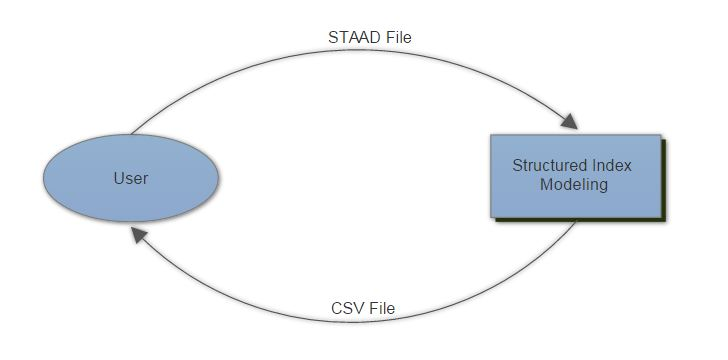
\includegraphics[width=0.7\linewidth]{images/image53.jpeg}
\caption{DFD level 0}
\label{fig:image1}
\end{figure}

\begin{figure}[!th]
\centering
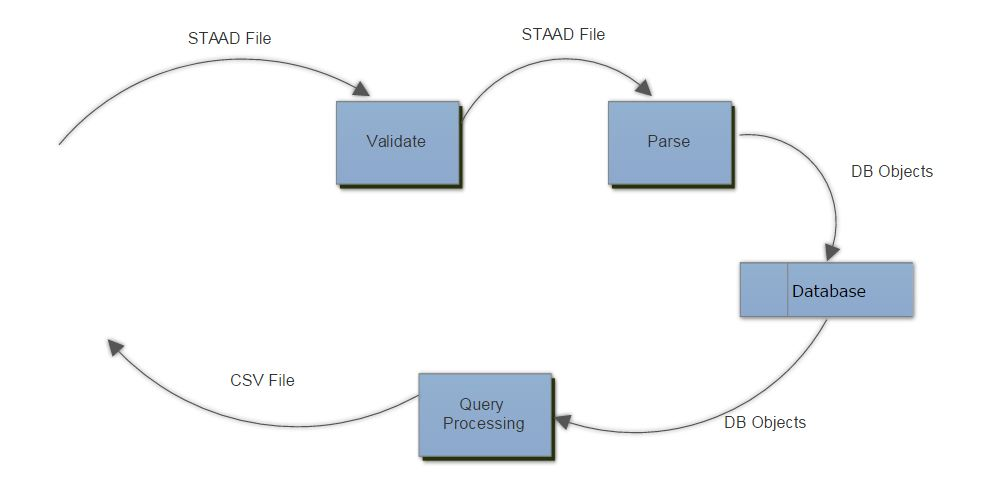
\includegraphics[width=0.7\linewidth]{images/image54.jpeg}
\caption{DFD level 1}
\label{fig:image1}
\end{figure}


{\centering\chapter*{Practical NO.5}

\section*{AIM: INTRODUCTION TO UML (UNIFIED MODELING LANGUAGE) AND UMBRELLO SOFTWARE}
}

The Unified Modelling Language (UML) is a general-purpose, developmental, modelling language in the field of software engineering that is intended to provide a standard way to visualize the design of a system.

	UML was originally motivated by the desire to standardize the disparate notational systems and approaches to software design developed by Grady Booch, Ivar Jacobson and James Rum Baugh at Rational Software in 1994?95, with further development led by them through 1996.

In 1997 UML was adopted as a standard by the Object Management Group (OMG), and has been managed by this organization ever since. In 2005 the Unified Modelling Language was also published by the International Organization for Standardization (ISO) as an approved ISO standard. Since then it has been periodically revised to cover the latest revision of UML

The Unified Modelling Language (UML) offers a way to visualize a system's architectural blueprints in a diagram (see image), including elements such as:

\begin{itemize}
\item Any activities (jobs) Individual components of the system
\item And how they can interact with other software components.
\item How the system will run
\item How entities interact with others (components and interfaces)
\item External user interface

\end{itemize}
Although originally intended solely for object-oriented design documentation, the Unified Modelling Language (UML) has been extended to cover a larger set of design documentation (as listed above), and been found useful in many contexts.

\subsection*{List of UML Diagram Types}
Types of UML diagrams with structure diagrams coming first and behavioural diagrams starting from position 8. Click on any diagram type to visit that specific diagram type?s description.
\begin{itemize}
\item Class Diagram
\item Component Diagram
\item Deployment Diagram
\item Object Diagram
\item Package Diagram 
\item Profile Diagram
\item Composite Structure Diagram
\item Use Case Diagram
\item Activity Diagram
\item Sequence Diagram

\end{itemize}
\subsection*{Class Diagram}
Class diagrams are arguably the most used UML diagram type. It is the main building block of any object oriented solution. It shows the classes in a system, attributes and operations of each class and the relationship between each class.

In most modelling tools, a class has three parts, name at the top, attributes in the middle and operations or methods at the bottom. In large systems with many related classes, classes are grouped together to create class diagrams. Different relationships between classes are shown by different types of arrowsClass Diagram

\begin{figure}[!th]
\centering
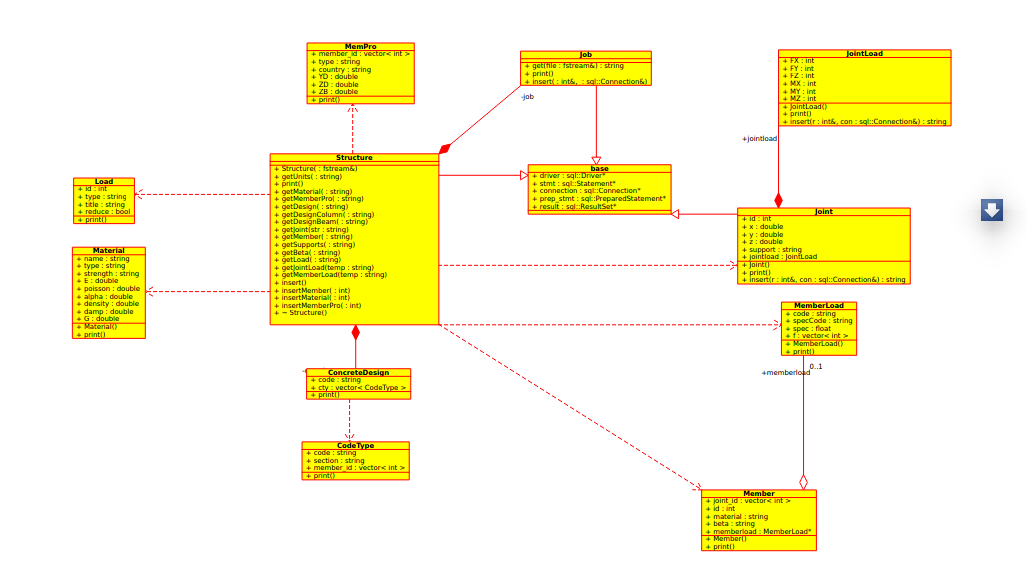
\includegraphics[width=1\linewidth]{images/image55.png}
\caption{class Diagram}
\label{fig:image1}
\end{figure}

\subsection*{Sequence diagram:} 
A Sequence diagram is an interaction diagram that shows how processes operate with one another and in what order. It is a construct of a Message Sequence Chart. A sequence diagram shows object interactions arranged in time sequence. It depicts the objects and classes involved in the scenario and the sequence of messages exchanged between the objects needed to carry out the functionality of the scenario. Sequence diagrams are typically associated with use case realizations in the Logical View of the system under development. Sequence diagrams are sometimes called event diagrams or event scenarios.
\begin{figure}[!th]
\centering
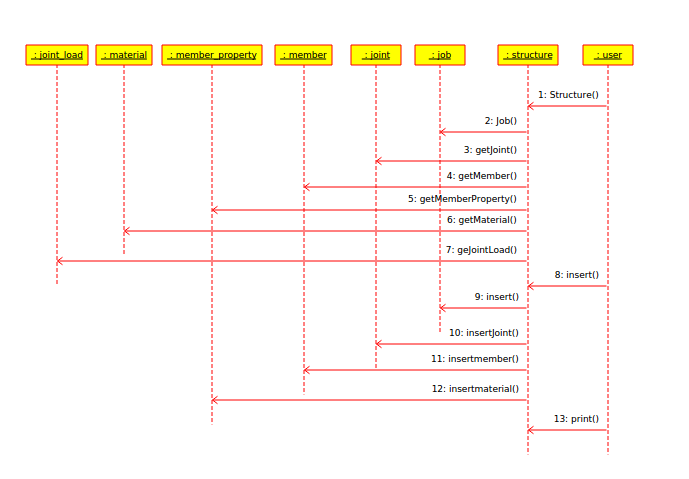
\includegraphics[width=1\linewidth]{images/image56.png}
\caption{Sequence diagram}
\label{fig:image1}
\end{figure}

\subsection*{Use Case Diagram}
As the most known diagram type of the behavioural UML diagrams, Use case diagrams give a graphic overview of the actors involved in a system, different functions needed by those actors and how these different functions are interacted.  	It?s a great starting point for any project discussion, because you can easily identify the main factors involved and the main processes of the system Activity diagram is another important diagram in UML to describe dynamic aspects of the system.
Activity diagram is basically a flow chart to represent the flow form one activity to another activity. The activity can be described as an operation of the system. So the control flow is drawn from one operation to another. This flow can be sequential, branched or concurrent. Activity diagrams deals with all type of flow control by using different elements like fork, join etc.

\begin{figure}[!th]
\centering
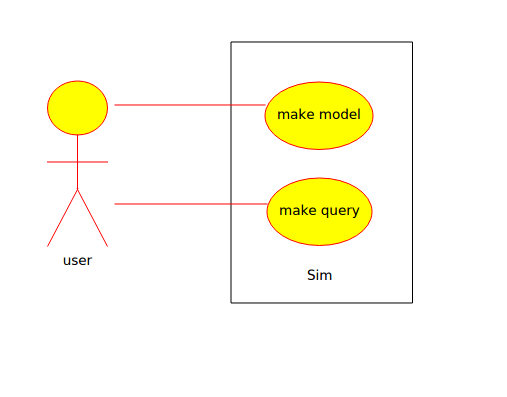
\includegraphics[width=1\linewidth]{images/image57.png}
\caption{Use Case Diagram}
\label{fig:image1}
\end{figure}

\subsection*{State chart diagram}
The name of the diagram itself clarifies the purpose of the diagram and other details. It describes different states of a component in a system. The states are specific to a component/object of a system.
A State chart diagram describes a state machine. Now to clarify it state machine can be defined as a machine which defines different states of an object and these states ,are controlled by external or internal events

\begin{figure}[!th]
\centering
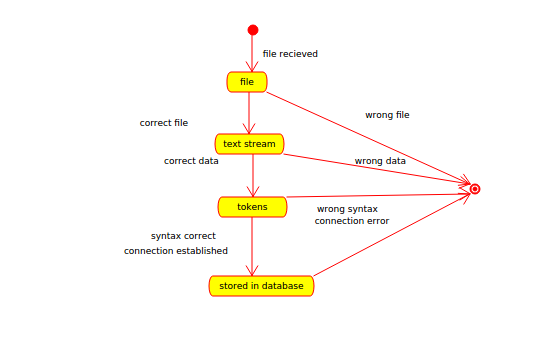
\includegraphics[width=1\linewidth]{images/image100.png}
\caption{Use Case Diagram}
\label{fig:image1}
\end{figure}


\subsection*{Umbrello software}
Umbrello UML Modeller is a Unified Modelling Language (UML) diagram program based on KDE Technology.
UML allows you to create diagrams of software and other systems in a standard format to document or design the structure of your programs.
You may take a look at the screenshots to see umbrello in action. Our handbook gives a good introduction to Umbrello and UML modelling.Umbrello comes with KDE SC, included with every Linux distribution and available through your package manager. See Installation to install Umbrello.

\newpage
\section*{AIM:Study and usage of any Design phase CASE Tool.}

CASE stands for Computer Aided Software Engineering. It means, development and maintenance of software projects with help of various automated software tools.

\subsection*{Case Tools:}
CASE tools are set of software application programs, which are used to automate SDLC activities. CASE tools are used by software project managers, analysts and engineers to develop software system.

There are number of CASE tools available to simplify various stages of Software Development Life Cycle such as Analysis tools, Design tools, Project Management Tools, Database Management tools, Documentation tools are to name a few.

Use of CASE tools accelerates the development of project to produce desired result and helps to uncover flaws before moving ahead with next stage in software development.

\subsubsection*{Components of CASE Tools:}
CASE tools can be broadly divided into the following parts based on their use at a particular SDLC stage:

\begin{itemize}


\item \textbf{Central Repository}
CASE tools require a central repository, which can serve as a source of common, integrated and consistent information. Central repository is a central place of storage where product specifications, requirement documents, related reports and diagrams, other useful information regarding management is stored. Central repository also serves as data dictionary.

\begin{figure}[!th]
\centering
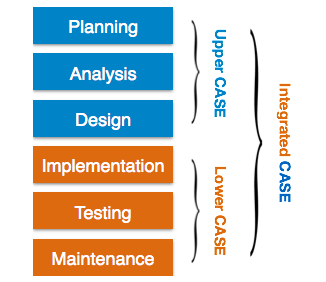
\includegraphics[width=1\linewidth]{images/image91.png}
\label{fig:image1}
\end{figure}

\item \textbf{Upper Case Tools}
Upper CASE tools are used in planning, analysis and design stages of SDLC.

\item \textbf{Lower Case Tools}
Lower CASE tools are used in implementation, testing and maintenance.

\item \textbf{Integrated Case Tools}
Integrated CASE tools are helpful in all the stages of SDLC, from Requirement gathering to Testing and documentation.

\end{itemize}
\subsubsection*{CASE Tools Types}

\begin{itemize}

\item \textbf{Diagram Tools}
These tools are used to represent system components, data and control flow among various software components and system structure in a graphical form. For example, Flow Chart Maker tool for creating state-of-the-art flowcharts.

\item \textbf{Process Modelling Tools}
Process modelling is method to create software process model, which is used to develop the software. Process modelling tools help the managers to choose a process model or modify it as per the requirement of software product. For example, EPF Composer.

\item \textbf{Project Management Tools}
These tools are used for project planning, cost and effort estimation, project scheduling and resource planning. Managers have to strictly comply project execution with every mentioned step in software project management.

\item \textbf{Documentation Tools}
Documentation tools generate documents for technical users and end users. Technical users are mostly in-house professionals of the development team who refer to system manual, reference manual, training manual, installation manuals etc. The end user documents describe the functioning and how-to of the system such as user manual. For example, Doxygen, DrExplain, Adobe RoboHelp for documentation.

\item \textbf{Analysis Tools}
These tools help to gather requirements, automatically check for any inconsistency, inaccuracy in the diagrams, data redundancies or erroneous omissions. For example, Accept 360, Accompa, CaseComplete for requirement analysis, Visible Analyst for total analysis.

\item\textbf{Design Tools}
These tools help software designers to design the block structure of the software, which may further be broken down in smaller modules using refinement techniques. These tools provides detailing of each module and interconnections among modules. For example, Animated Software Design.

\item \textbf{Change Control Tools}
These tools are considered as a part of configuration management tools. They deal with changes made to the software after its baseline is fixed or when the software is first released. CASE tools automate change tracking, file management, code management and more. It also helps in enforcing change policy of the organization.

\item \textbf{Programming Tools}
These tools consist of programming environments like IDE (Integrated Development Environment), in-built modules library and simulation tools. These tools provide comprehensive aid in building software product and include features for simulation and testing. For example, Cscope to search code in C, Eclipse.

\end{itemize}

\subsubsection*{Points of CASE Tools}
\begin{enumerate}
\item They provides better perceptive of system. 
\item Facilitates communication among team members. 
\item Tools are more effective for large scale systems and immense projects. 
\item CASE tools provide visibility of processes and logic. 
\item CASE tools improve quality and productivity of software. 
\item CASE tools reduce the time for error correction and maintenance. 
\item CASE tools provide clear readability and maintainability of the system.
\end{enumerate}


\subsubsection*{ Factor influencing the success of CASE}
CASE tools facing many troubles in creating a suitable place in market e.g.
\begin{enumerate}
\item Even after the completion of the design it is not necessary that it will fulfill the requirements. 
\item Though CASE tools are helpful for the developer but do not assure that the design is according to the requirements. 
\item Good quality CASE tools are very expensive and prove costly for the development. 
\item CASE tools also required training for the user that increase the overall cast of development. 
\item Almost every tool has its limitation that decreases its use and popularity. 
\item Some tools may have very limited functionality and may not address all possible domain activities. 
\item Every tool has a specific methodology for designing and modelling of the system. Due to this you?re bound to follow them that decrease the flexibility which decrease the use of CASE tools. 
\item Frequent users get used to it and afterward developers try to use the same approach and tool for other projects whether the tool addresses the target projects problems or not.
\end{enumerate} 


\subsubsection*{Use of CASE Tools}
The purpose of CASE is to reduce the cost and time required for the system development and the focus is on the quality of the end product. CASE is not being used as it was being expected. Most of the companies are reluctant to adopt the CASE tools. It is observed that CASE is being used but not in many companies.The reasons for abandonment included cost, lack of measurable returns, and unrealistic expectations. Organizations that used CASE tools and found that large numbers of their systems developers were not using CASE tools. He reported that in 57\% of the organizations surveyed that were using CASE tools, less than 25\% of the systems developers used the tools (Diane Lending 1998). And in those companies where CASE is adopted only few people are using CASE tools. In a survey of 67 companies it has been observed that 69\% companies had never used CASE tools. And those people who are using CASE tools admitted that the use of CASE tools improved the standard of documentation and in result the system was easier to test and maintain. But people who used CASE tools also admitted that using CASE tools requires more time and effort and also adds in overall development time. 

Less than 30\% of the potential users and developers use the CASE and those who use it, uses the simplest and basic functionality of the CASE tools. This shows that even after getting so much popular CASE tools are not adopted and used so much in the software development industry as they expected or as they should be used. Just after one year of introduction 70\% of CASE tools are never used, 20 are used by one group and 5\% of CASE tools are used in general [Juhani Iivar,1996].It has been observed that CASE Tools are not being used from the time CASE got recognition. CASE is being approached experimentarily and involves a very long learning curve.

\subsubsection*{Conclusion}
CASE tools plays an important role in Software Development and getting its appreciation in software development industry slowly but surly. But CASE is still in growth and there are different perceptions about CASE.CASE tools are not being used as they are expected to. Though, there are many new CASE tools available in the market and integrated CASE tools provides significant help and support for developers and programmers throughout SDLC in design and development activities but CASE tools have never been first choice for the majority of developers. Research about CASE usage in different organizations has shown that CASE is not always welcomed by developers and programmers and has never been as a tool of choice in organizations. And where CASE is used, the developers are using only minimal required functionality.

{\centering\chapter*{Practical NO.6}

\section*{AIM: Preparation of Software Configuration Management
and Risk Management related documents}
}
The purpose of Software Configuration Management is to establish and maintain the integrity

of the products of the software project throughout the project's software life cy
cle. Software
Configuration Management involves identify
ing configuration items for the software project,
controlling these configuration items and changes to them, and recording and reporting status
and change activity
 for these configuration items.
 
Configuration management (CM) refers to a discipline for evaluating, coordinating,
approving or disapproving, and implementing changes in artefacts that are used to construct
and maintain software sy
stems. An artifact may
 be a piece of hardware or software or
documentation. CM enables the management of artifact from the initial concept through
design, implementation, testing, base lining, building, release, and maintenance.

CM is intended to eliminate the confusion and error brought about by
 the existence of
different versions of artifacts. Artifact change is a fact of life: plan for it or plan to be
overwhelmed by
 it. Changes are made to correct errors, provide enhancements, or simply

reflect the evolutionary
 refinement of product definition. CM is about keeping the inevitable
change under control. Without a well-enforced CM process, different team members
(possibly
 at different sites) can use different versions of artifacts unintentionally
; individuals
can create versions without the proper authority
; and the wrong version of an artifact can be
used inadvertently
. Successful CM requires a well-defined and institutionalized set of policies
and standards that clearly
 define
\begin{itemize}

\item The set of artifacts (configuration items) under the jurisdiction of CM (Models that
will be used)
\item
How artifacts are named (division of models into admin, student and company

module)
\item How artifacts enter and leave the controlled set (various logins and logouts)
\item How an artifact under CM is allowed to change (admin has the sole authority
)\item
How different versions of an artifact under CM are made available and under what
conditions each one can be used (whether to register , participate or work as admin)
\item
How CM tools are used to enable and enforce CM
\end{itemize}
These policies and standards are documented in a CM plan that informs every
one in the
organization just how CM is carried out.
Aspects Peculiar to Product Lines
CM is, of course, an integral part of any
 software development activity
, but it takes on a
special significance in the product line context. As illustrated in the following figure, CM for
product lines is generally
 viewed as a multidimensional version of the CM problem for one-
of-a-kind sy
stems.
Configuration Management and Software Product Lines
The core assets constitute a configuration that needs to be managed, each product in the
product line constitutes a configuration that must be managed, and the management of all
these configurations must be coordinated under a single process.
CM for product lines is therefore more complex than it is for single sy
stems. CM capabilities
such as parallel development, distributed engineering, build and release management, change
management, configuration and workspace management, and process management must be
supported by
 the tools, processes, and environments put in place for CM in a product line
context.
\begin{itemize}

\item In single-sy
stem CM, each version of the sy
stem has a configuration associated with it that
defines the versions of the configuration items that went into that sy
stem's production. In
product line CM, a configuration must be maintained for each version of each product.
\item In single-sy
stem CM, each product with all of its versions may
 be managed separately
. In
product line CM, such management is untenable, because the core assets are used across
all products. Hence, the entire product line is usually
 managed with a single, unified CM
process.
\item Product line CM must control the configuration of the core asset base and its use by
 all
product developers. It must account for the fact that core assets are usually
 produced by
one team and used in parallel by
 several others. Single-sy
stem CM has no such burden:
the component developers and product developers are the same people.
\item Only
 the most capable CM tools can be used in a product line effort. Many
 tools that are
adequate for single-sy
stem CM are simply
 not sufficiently
 robust to handle the demands
of product line CM. (See the "Tool Support" practice area for a more complete
discussion of tools.)


\end{itemize}

The mission of product line CM is allowing the rapid reconstruction of any
 product version
that may
 have been built using various versions of the core assets and development/operating
environment plus various versions of product-specific artifacts. One product line manager
summed up the problem this way
: "Sometime, in the middle of the night, one of y
our
customers is going to call y
ou and tell y
ou that his version of one of y
our products doesn't
work. You are going to have to duplicate that product in y
our test lab before y
ou can begin to
troubleshoot.
\subsection*{Risk Management Plan:}
\subsubsection*{Purpose of the Risk management plan}

A risk is an event or condition that, if it occurs, could have a positive or negative effect on a
project?s objectives. Risk Management is the process of identify
ing, assessing, responding to,
monitoring, and reporting risks. This Risk Management Plan defines how risks associated
with the <Project Name> project will be identified, analy
zed, and managed. It outlines how
risk management activities will be performed, recorded, and monitored throughout the
lifecy
cle of the project and provides templates and practices for recording and prioritizing
risks.

The Risk Management Plan is created by
 the project manager in the Planning Phase of the
CDC Unified Process and is monitored and updated throughout the project. The intended
audience of this document is the project team, project sponsor and management.
\subsubsection*{Risk management Procedure:}
The project manager working with the project team and project sponsors will ensure that risks
are actively
 identified, analy
zed, and managed throughout the life of the project. Risks will be
identified as early
 as possible in the project so as to minimize their impact. The steps foraccomplishing this are outlined in the following sections. The <project manager or other
designee> will serve as the Risk Manager for this project.
\subsubsection*{Risk Identification}
Risk identification will involve the project team, appropriate stakeholders, and will include an
evaluation of environmental factors, organizational culture and the project management plan
including the project scope. Careful attention will be given to the project deliverables,
assumptions, constraints, WBS, cost/effort estimates, resource plan, and other key
 project
documents.

A Risk Management Log will be generated and updated as needed and will be stored
electronically
 in the project library
 located at <file location>

In our project Function Organiser also we looked at various aspects of risks that could occur.
We looked at the environmental factors and our organizational culture pertained to the student
body
 of the college

Project scope included serving and notifications of various events for which the students
registered, so that it reduces the manual work and the sy
stem of organizing events could
come easy
. Assumptions of student body
 and companies that would participate and cost of
project was also designed.
\subsubsection*{Risk Analysis}
All risks identified will be assessed to identify
 the range of possible project outcomes.
Qualification will be used to determine which risks are the top risks to pursue and respond to
and which risks can be ignored Qualitative Risk Analy
sis



The probability
 and impact of occurrence for each identified risk will be assessed by
 the
project manager, with input from the project team using the following approach:
\begin{description}
\item{Probability}

\begin{itemize}
\item \textbf{High} Greater than 70 probability
 of occurrence
\item\textbf{ Medium} Between 30 and 70 probability
 of occurrence
\item \textbf{Low} Below 30 probability
 of occurrence
\end{itemize}

\item{Impact}

\begin{itemize}

\item \textbf{High} Risk that has the potential to greatly
 impact project cost, project schedule or
performance (problem in working of registration window as in case of our project)
\item\textbf{ Medium } Risk that has the potential to slightly
 impact project cost, project schedule
or performance (students not aware of the functionality
 of the project Function
Organiser.
\item \textbf{Low} Risk that has relatively
 little impact on cost, schedule or Performance
(connection or connectivity
 issues as in terms of the project)

 \end{itemize}
 
 \end{description}
Risks that fall within the RED and YELLOW zones will have risk response planning which
may
 include both a risk mitigation and a risk contingency
 plan.
\subsubsection*{Quantitative Risk Analysis}
Analy
sis of risk events that have been prioritized using the qualitative risk analy
sis process
and their effect on project activities will be estimated, a numerical rating applied to each risk
based on this analy
sis, and then documented in this section of the risk management plan.

{\centering\chapter*{Practical NO.7}
\section*{AIM: To perform unit testing and integration testing.}
}
\subsection*{Unit Testing}
In computer programming, unit testing is a software testing method by which individual units of source code, sets of one or more computer program modules together with associated control data, usage procedures, and operating procedures are tested to determine if they are fit for use. Intuitively, one can view a unit as the smallest testable part of an application. In procedural programming, a unit could be an entire module, but it is more commonly an individual function or procedure. In object-oriented programming, a unit is often an entire interface, such as a class, but could be an individual method. Unit tests are short code fragments created by programmers or occasionally by white box testers during the development process. Ideally, each test case is independent from the others. Substitutes such as method stubs, mock objects, fakes, and test harnesses can be used to assist testing a module in isolation. Unit tests are typically written and run by software developers to ensure that code meets its design and behaves as intended. 

\begin{figure}[!th]
\centering
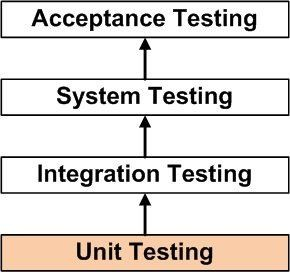
\includegraphics[width=0.3\linewidth]{images/image92.jpg}
\caption{Testing}
\end{figure}


Unit Testing is performed by using the White Box Testing method.

\subsection*{TASKS of unit test}
\begin{itemize}
\item Unit Test Plan
\begin{itemize}

\item Prepare

\item Review  
\item
Rework
\item
Baseline

\end{itemize}
 

\item Unit Test Cases/Scripts 

\begin{itemize}
\item Prepare

\item Review

\item
Rework

\item
Baseline

\end{itemize}

\item Unit Test
\begin{itemize}
\item Perform
\end{itemize}

\end{itemize}
\subsection*{Benefits of Unit testing}
The goal of unit testing is to isolate each part of the program and show that the individual parts are correct. A unit test provides a strict, written contract that the piece of code must satisfy. As a result, it affords several benefits.



\subsection*{Integration Testing}
To perform integration testing, first, all unit testing has to be completed. Upon completion of unit testing, integration testing begins. Integration testing is black box testing. The purpose of integration testing is to ensure distinct components of the application still work in accordance to customer requirements. Test cases are developed with the express purpose of exercising the interfaces between the components. This activity is carried out by the test team. Integration testing is considered complete, when actual results and expected results are either in line or differences are explainable, or acceptable, based on client input. 

\begin{itemize}
\item[step1] 
\textbf{Identify Unit Interfaces}: The developer of each program unit identifies and documents the unit's interfaces for the Responding to queries from terminals for information, Managing transaction data entered for processing, Obtaining, updating or creating transactions on computer files , Passing or receiving information from other logical processing units, Sending  messages to terminals, Providing the results of processing to some output device or unit

\item[Step 2]\textbf{
 Reconcile Interfaces for Completeness}: The information needed for the integration test template is collected for all program units in the software being tested. Whenever one unit interfaces with another, those interfaces are reconciled. For example, if program unit A transmits data to program unit B, program unit B should indicate that it has received that input from program unit A. Interfaces not reconciled are examined before integration tests are executed. 
 
\item[Step 3]
\textbf{Create Integration Test Conditions}: One or more test conditions are prepared for integrating each program unit. After the condition is created, the number of the test condition is documented in the test template.  

\item[Step 4]\textbf{
Evaluate the Completeness of Integration Test Conditions}: The following list of questions will help guide evaluation of the completeness of integration test conditions recorded on the integration testing template. This list can also help determine whether test conditions created for the integration process are complete.

\end{itemize}

\begin{table}
\caption{unit testing}
\begin{tabular}{|p{1cm}|p{2cm}|p{3cm}|p{2cm}|p{2cm}|p{3cm}|p{1.2cm}|} 
\hline
Test Case ID & Test Case Name & Description & Pre-Condition
 & Execution Step & Expected Result
 & Status \\ 
\hline \rule[-2ex]{0pt}{5.5ex} Ek001 & Network 
Test 
& The system works over a network through a web interface hence the first test is to check if there is proper transferring of the required data over the network.
& 1. Proper Network access.\newline
 2. Correct working URL for the SIM system.
 & 1. Open the web browser and open the SIM executable file using localhost.\newline
   2. Upload a file or open an existing project to see if the system is working.
& The System should work properly using the web browser and all of its offered options shall work properly. &  passed\\ 
\hline \rule[-2ex]{0pt}{5.5ex} Ek002 &
File Exist 
Test
  & 
  The file uploaded by the user must exist for the system to further parse and store it. This test checks for that.
  &
  1. The file must be of .STD format.\newline
  2. The file selected by the user must be supplied in full and no network issues shall halt this process.
  &1. Select the upload file option from the home page.\newline
  2. Upload the file with proper location and address of the file.
  &The system shall generate appropriate error message if the selected file does not exist in the user?s computer. Otherwise proper functioning of the system is assumed.
   &  passed\\ 
   
\hline 
\end{tabular} 

\end{table}
\begin{table}[t]
\caption{unit testing}

\begin{tabular}{|p{1cm}|p{2cm}|p{3cm}|p{2cm}|p{2cm}|p{3cm}|p{1.2cm}|} 
\hline
Test Case ID & Test Case Name & Description & Pre-Condition
 & Execution Step & Expected Result
 & Status \\ 
\hline \rule[-2ex]{0pt}{5.5ex}  Ek003 & 
File Valid
Test
 &  The file provided by the user may be in simple text form but the data inside the file must be in strict accordance to the STAAD PRO file otherwise the system must handle the wrong format of the input data.
 & 1. File must be uploaded completely.\newline
 2. It must be of .STD extension.
& 1. Select the upload file option from the home page.\newline
 2. Upload any file from your system.
 & In case the selected file is not of the right extension or the contents of the file are in accordance to the rules of STAAD PRO, then the system shall report the error via a message and return to the home page. Otherwise usual functioning shall proceed.
 &  passsed\\ 
\hline \rule[-2ex]{0pt}{5.5ex}  Ek004 &
Database 
Test
 & Database 
 Test
 Things that are parsed by the system and converted in Database object form are needed to be stored in the database back at the server end, this tests checks if this is working properly.
 & 1. The parsing of the file must execute correctly.\newline
 2. Proper database administration rights must be awarded.\newline
 3. The storage space must be sufficient.\newline
 & 1. Upload a correct STAAD PRO file or open an existing project.\newline
 2. Restart the parsing process for the selected/uploaded file.\newline
 3. Save the parsed contents into a new database entry.
 & The valid file should be parsed properly and to completion. No information in the file shall be skipped and no false information shall be assumed. Every result parsed shall be stored in the database under proper file names and corresponding structure identities and Job Id?s.
  & passsed\\ 
\hline 
\end{tabular} 
\end{table}
\begin{table}[t]
\caption{table for integration testing}
\begin{tabular}{|p{1cm}|p{2cm}|p{3cm}|p{2cm}|p{2cm}|p{3cm}|p{1.2cm}|} 
\hline
Test Case ID & Test Case Name & Description & Pre-Condition
 & Execution Step & Expected Result
 & Status \\ 

 
\hline \rule[-2ex]{0pt}{5.5ex}  MA001 & Converting a STAAD PRO file into a Database file.
& A file when loaded and validated by the system is parsed by the system and the parsed elements are stored in the database. This is about half the job. 
& The network should be working properly and the file should be with correct form and syntax.
&
 
1. Select the upload option from the home page.\newline
2. Upload a file.\newline
3. Perform the parsing to completion.\newline
4. Store the result in the database.\newline

& After the test, an equivalent database and csv file is generated at the specified location on the computer.
&
Passed \\
\hline

\rule[-2ex]{0pt}{5.5ex}  MA002 & Converting a Database file into a STAAD PRO file.
& A file when loaded and validated by the system is parsed by the system and the parsed elements are stored in the database. This is about half the job. The other half comprises of actually recreating the entire file from only the information stored in the database. This is like performing a query of the highest level on the database.
& The network should be working properly and the file should be with correct form and syntax.
&
 
1. Select the upload option from the home page.\newline
2. Upload a file.\newline
3. Perform the parsing to completion.\newline
4. Store the result in the database.\newline
5. Delete the original file.\newline
6. Retrieve the file from the database
\newline
& After the test, an equivalent STAAD PRO file is generated at the specified location on the computer.
&
Passed \\
 

\hline

\end{tabular} 



\end{table}



{\centering\chapter*{Practical No.8}
\section*{AIM: To perform various white box and black box testng techniques.}
}

\subsection*{White Box Testing Technique}
White-box testing (also known as clear box testing, glass box testing, transparent box testing, and structural testing) is a method of testing software that tests internal structures or workings of an application, as opposed to its functionality (i.e. black-box testing). In white-box testing an internal perspective of the system, as well as programming skills, are used to design test cases. The tester chooses inputs to exercise paths through the code and determine the appropriate outputs. This is analogous to testing nodes in a circuit, e.g. in-circuit testing (ICT).
 
White-box testing can be applied at the unit, integration and system levels of the software testing process. Although traditional testers tended to think of white-box testing as being done at the unit level, it is used for integration and system testing more frequently today. It can test paths within a unit, paths between units during integration, and between subsystems during a system level test. Though this method of test design can uncover many errors or problems, it has the potential to miss unimplemented parts of the specification or missing requirements. 
White-box test design techniques include the following code coverage criteria: 

\begin{itemize}


\item	Control flow testing 
\item	Data flow testing 
\item	Branch testing 
\item	Statement coverage 
\item	Decision coverage 
\item	Modified condition/decision coverage 
\item	Prime path testing 
\item	Path testing 
\end{itemize}

\subsubsection*{Basic Procedures}
 White-box testing's basic procedures involve the understanding of the source code that you are testing at a deep level to be able to test them. The programmer must have a deep understanding of the application to know what kinds of test cases to create so that every visible path is exercised for testing. Once the source code is understood then the source code can be analyzed for test cases to be created. These are the three basic steps that white-box testing takes in order to create test cases: 
 
 \begin{itemize}

\item Input involves different types of requirements, functional specifications, detailed designing of documents, proper source code, security specifications. This is the preparation stage of white-box testing to layout all of the basic information. 
\item Processing involves performing risk analysis to guide whole testing process, proper test plan, execute test cases and communicate results. This is the phase of building test cases to make sure they thoroughly test the application the given results are recorded accordingly. 
\item Output involves preparing final report that encompasses all of the above preparations and results. 

 
 \end{itemize}
\subsubsection*{Advantages}
White-box testing is one of the two biggest testing methodologies used today. It has several major advantages: 
\begin{itemize}
\item Side  effects of having the knowledge of the source code is beneficial to thorough testing.
\item  Optimization of code by revealing hidden errors and being able to remove these possible defects.  
\item  Gives the programmer introspection because developers carefully describe any new implementation.  
\item  Provides traceability of tests from the source, allowing future changes to the software to be easily captured in changes to the tests.  
\item  White box tests are easy to automate.  
\item  White box testing give clear, engineering-based, rules for when to stop testing.  

\end{itemize}

\subsubsection*{Disadvantages}
Although white-box testing has great advantages, it is not perfect and contains some disadvantages: 
\begin{itemize}
\item White-box testing brings complexity to testing because the tester must have knowledge of the program, including being a programmer. White-box testing requires a programmer with a high-level of knowledge due to the complexity of the level of testing that needs to be done. 
\item On some occasions, it is not realistic to be able to test every single existing condition of the application and some conditions will be untested.  
\item The tests focus on the software as it exists, and missing functionality may not be discovered. 

\end{itemize}

\subsection*{Black Box Testing Technique}
Black-box testing is a method of software testing that examines the functionality of an application without peering into its internal structures or workings. This method of test can be applied to virtually every level of software testing: unit, integration, system and acceptance. It typically comprises most if not all higher level testing, but can also dominate unit testing as well. 

\subsubsection*{Test Cases}
Test cases are built around specifications and requirements, i.e., what the application is supposed to do. Test cases are generally derived from external descriptions of the software, including specifications, requirements and design parameters. Although the tests used are primarily functional in nature, non-functional tests may also be used. The test designer selects both valid and invalid inputs and determines the correct output without any knowledge of the test object's internal structure. 

\subsubsection*{Test design techniques}
Typical black-box test design techniques include:
\begin{itemize}
\item	Decision table testing 
\item	 All-pairs testing 
\item	State transition analysis  
\item	Equivalence partitioning 
\item	Boundary value analysis 
\item	Cause�effect graph 
\item	Error guessing.

\end{itemize} 


\begin{figure}[!th]
\centering
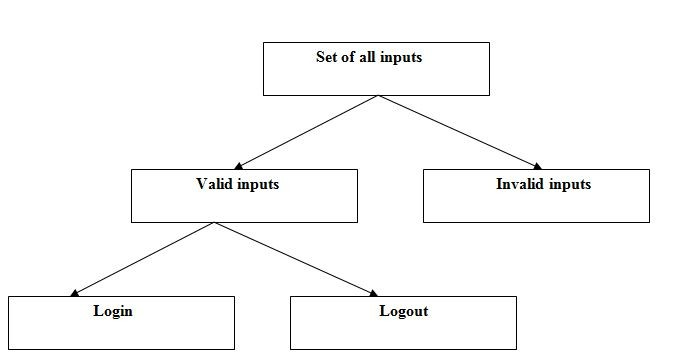
\includegraphics[width=0.7\linewidth]{images/image93.jpg}
\caption{Black Box Testing}
\end{figure}



{\centering\chapter*{Practical No.9}
\section*{AIM: System testing of software.}
}

\subsection*{Requirement}
The software to be designed will create an index model for a 3 dimensional civil structure like a building or any other civil engineering project. This requires a software for designing such structures using a computer, the one used in SIM is STAAD PRO. In STAAD PRO the engineer draws the structure using various graphical tools and accordingly a .STD file is created that has all information about the building structure. Alternatively the engineer can choose to work from this file only and creating the elements of the building by writing pre-defined instructions into the file just like a script. It is this file that serves as the fundamental requirement for SIM. SIM parses this file and stores the parsed information into a database which is of object orientation nature.

SIM will serve multiple users at a time. This is achieved by providing a web interface to things so that various user can access it from their web browsers. The user is required to make a decision at the home page of whether to upload a new file or open an already uploaded file. If the user chooses the former then the user must provide with a valid and complete STAAD PRO file for the system to further process.  SIM must be able to provide the following services to the users:
\begin{enumerate}
\item The user must be able to change the working file without having to restart the system every time. This means that there must be navigational features in the system to move back and forth with different files in the same session.
\item The file provided by the user maybe half complete and/or with errors or outright empty. So the system must be able recognize these issues and offer the correct error message in response.
\item The user must be able to apply queries on the information stored in the databases. 
\item Just like in a query when the user retrieves certain information about the structure from the database, the user should be able if he/she wishes to, construct a whole, complete file from the information stored in the database.
\end{enumerate}

A user must be able to abort a file in processing at any time i.e. at the time of uploading as well as parsing. 

SIM communicates with the database back at the server end and interact to store and retrieve information. A processing of the file is considered complete only if all of the file has been parsed, it database objects has been created by the corresponding function and the objects have been properly transferred to the database at the back end. If this is not the case then no changes shall be made to the database and its consistent state must be maintained.

If the system recognizes that the file in consideration is not correct then it must point that out to the user and also be able to tell that in what manner is the file wrong. For example, if the file is wrong syntactically then the correct syntactic suggestion must be provided to the user.  If the file is not complete then simply a message must be passed to the user.

\begin{table}
\caption{table for integration testing}
\begin{tabular}{|p{1.5cm}|p{2cm}|p{5cm}|p{5cm}|p{1.5cm}|} 
\hline
Test Case ID & Test Case Name & Description & Expected Result
 & Status \\ 

 
\hline \rule[-2ex]{0pt}{5.5ex}  MA001 & Change file &
 The user must be able to change the working file without having to restart the system every time. This means that there must be navigational features in the system to move back and forth with different files in the same session.
& Without having to create a new session the user must be able to change the working files.
&
Passed \\
\hline

\rule[-2ex]{0pt}{5.5ex}  MA002 & valid file
&
The file provided by the user maybe half complete and/or with errors or outright empty. So the system must be able recognize these issues and offer the correct error message in response.
& The system must accept those files that are correct and complete otherwise proper redirection to the home page with an error message must be provided.

&
Passed \\

\hline
 
\rule[-2ex]{0pt}{5.5ex}  MA003 & query proccessing
&
The user must be able to apply queries on the information stored in the databases. 
&
All user queries that are valid must be answered properly
&
Passed \\
 
 \hline
 \rule[-2ex]{0pt}{5.5ex}  MA004 & File retrival
 & 
 Just like in a query when the user retrieves certain information about the structure from the database, the user should be able if he/she wishes to, construct a whole, complete file from the information stored in the database.
 
 & The whole file must be created from the informtion in the database &
 Passed \\
  

\hline

\end{tabular}
\end{table}

\begin{figure}[]
\centering
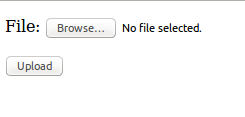
\includegraphics[width=0.7\linewidth]{images/image101.png}
\label{fig:image1}
\caption{Main screen}
\end{figure}
\begin{figure}[!ht]
\centering
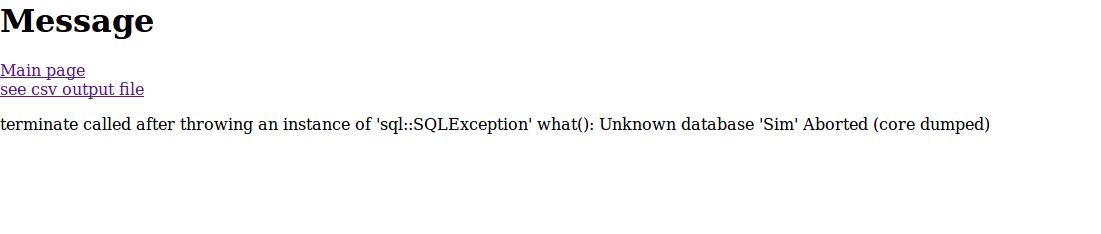
\includegraphics[width=1\linewidth]{images/102.png}
\label{fig:image1}
\caption{Message}
\end{figure}
\end{document}


